%%%%%%%%%%%%%%%%%%%%%%%%%%%%%%%%%% Beamer-Presentation 2022 %%%%%%%%%%%%%%%%%%%%%%%%%%%%%%%%%
\documentclass[12pt]{beamer}
%%%%%%%%%%%%%%%%%%%%%%%%%%%%%%%%%%%%%%%%%%%%%%%%%%%%%%%%%%%%%%%%%%%%%%%%%%%%%%%%%%%%%%
%\usepackage{pgfpages}
%\pgfpagesuselayout{4 on 1}[a4paper, border shrink=5mm, landscape]
\usepackage[T1]{fontenc}
\usepackage{ragged2e}\justifying
\usepackage{txfonts}
\usepackage{booktabs}
\usepackage{natbib}
\usepackage{bibentry}
\usepackage{appendixnumberbeamer}
\usepackage{pifont}
\usepackage{fontawesome}
\usepackage{textpos}
\usepackage{media9}
\usepackage{tikz}
%\usepackage{multirow}
\usepackage{multicol}
%\usepackage{amsmath}
\usepackage[compat=1.1.0]{tikz-feynman}
%=================================== Themes ==============================================
\usetheme{default}
% \useoutertheme[footline=authortitle,subsection=false]{miniframes} % Alternatively: miniframes, infolines, split
% \useinnertheme{circles}
\usefonttheme{serif}
%==================================== Preamble ==========================================
% \include{settings/preamble}
%=============================== Title information ======================================
\title{Overtraining}
%\subtitle{Write the subtitle}

% \author[Shubhajit Sana \hspace{4 pt} (Guide: Prof. J. Libby)]{Shubhajit Sana\\  Roll: PH18B004\\ Guide: Prof. James F. Libby\\[5mm] 
% \includegraphics[scale=0.04]{logo1}
% \hspace{2 cm}
% \includegraphics[width=1.8cm]{logo2}
% }

% \institute[IIT Madras]{Department of Physics,\\ Indian Institute of Technology Madras, \\ Chennai 600036, India}

%\date[\tiny \today]{\scriptsize \today}
% \date{November 22, 2022}

%\titlegraphic{\includegraphics[scale=0.08]{logo}}
% \logo{\includegraphics[scale=0.04]{logo}}

%=================================== Main body========================================
\beamertemplatenavigationsymbolsempty
\begin{document}

%--------------------------------------------------------------------------
% \section[Outline]{}
%-------------------------------------------------------------------------

%% TOC
% \begin{frame}{Outline}
% 	\tableofcontents	
% \end{frame}
			

% \begin{frame}{ variables}
% \hspace{-1in}
% \includegraphics[width=1.25\textwidth]{evaluate_/importance.pdf}
% 	\vspace{-3.3in}
% 	\begin{columns}
% 		\column{0.7\textwidth}
% 		\begin{figure}
% 			\includegraphics[width=1.0\textwidth]{evaluate_/diagonal_plot_test.pdf}
% 			\includegraphics[width=1.0\textwidth]{evaluate_/overtraining_plot_-6845103939654726996.pdf}
% 		\end{figure}
		
% 		\column{0.3\textwidth}
% 		% \begin{figure}
% 		% 	% \vspace{-0.2 in}
% 		% 	% 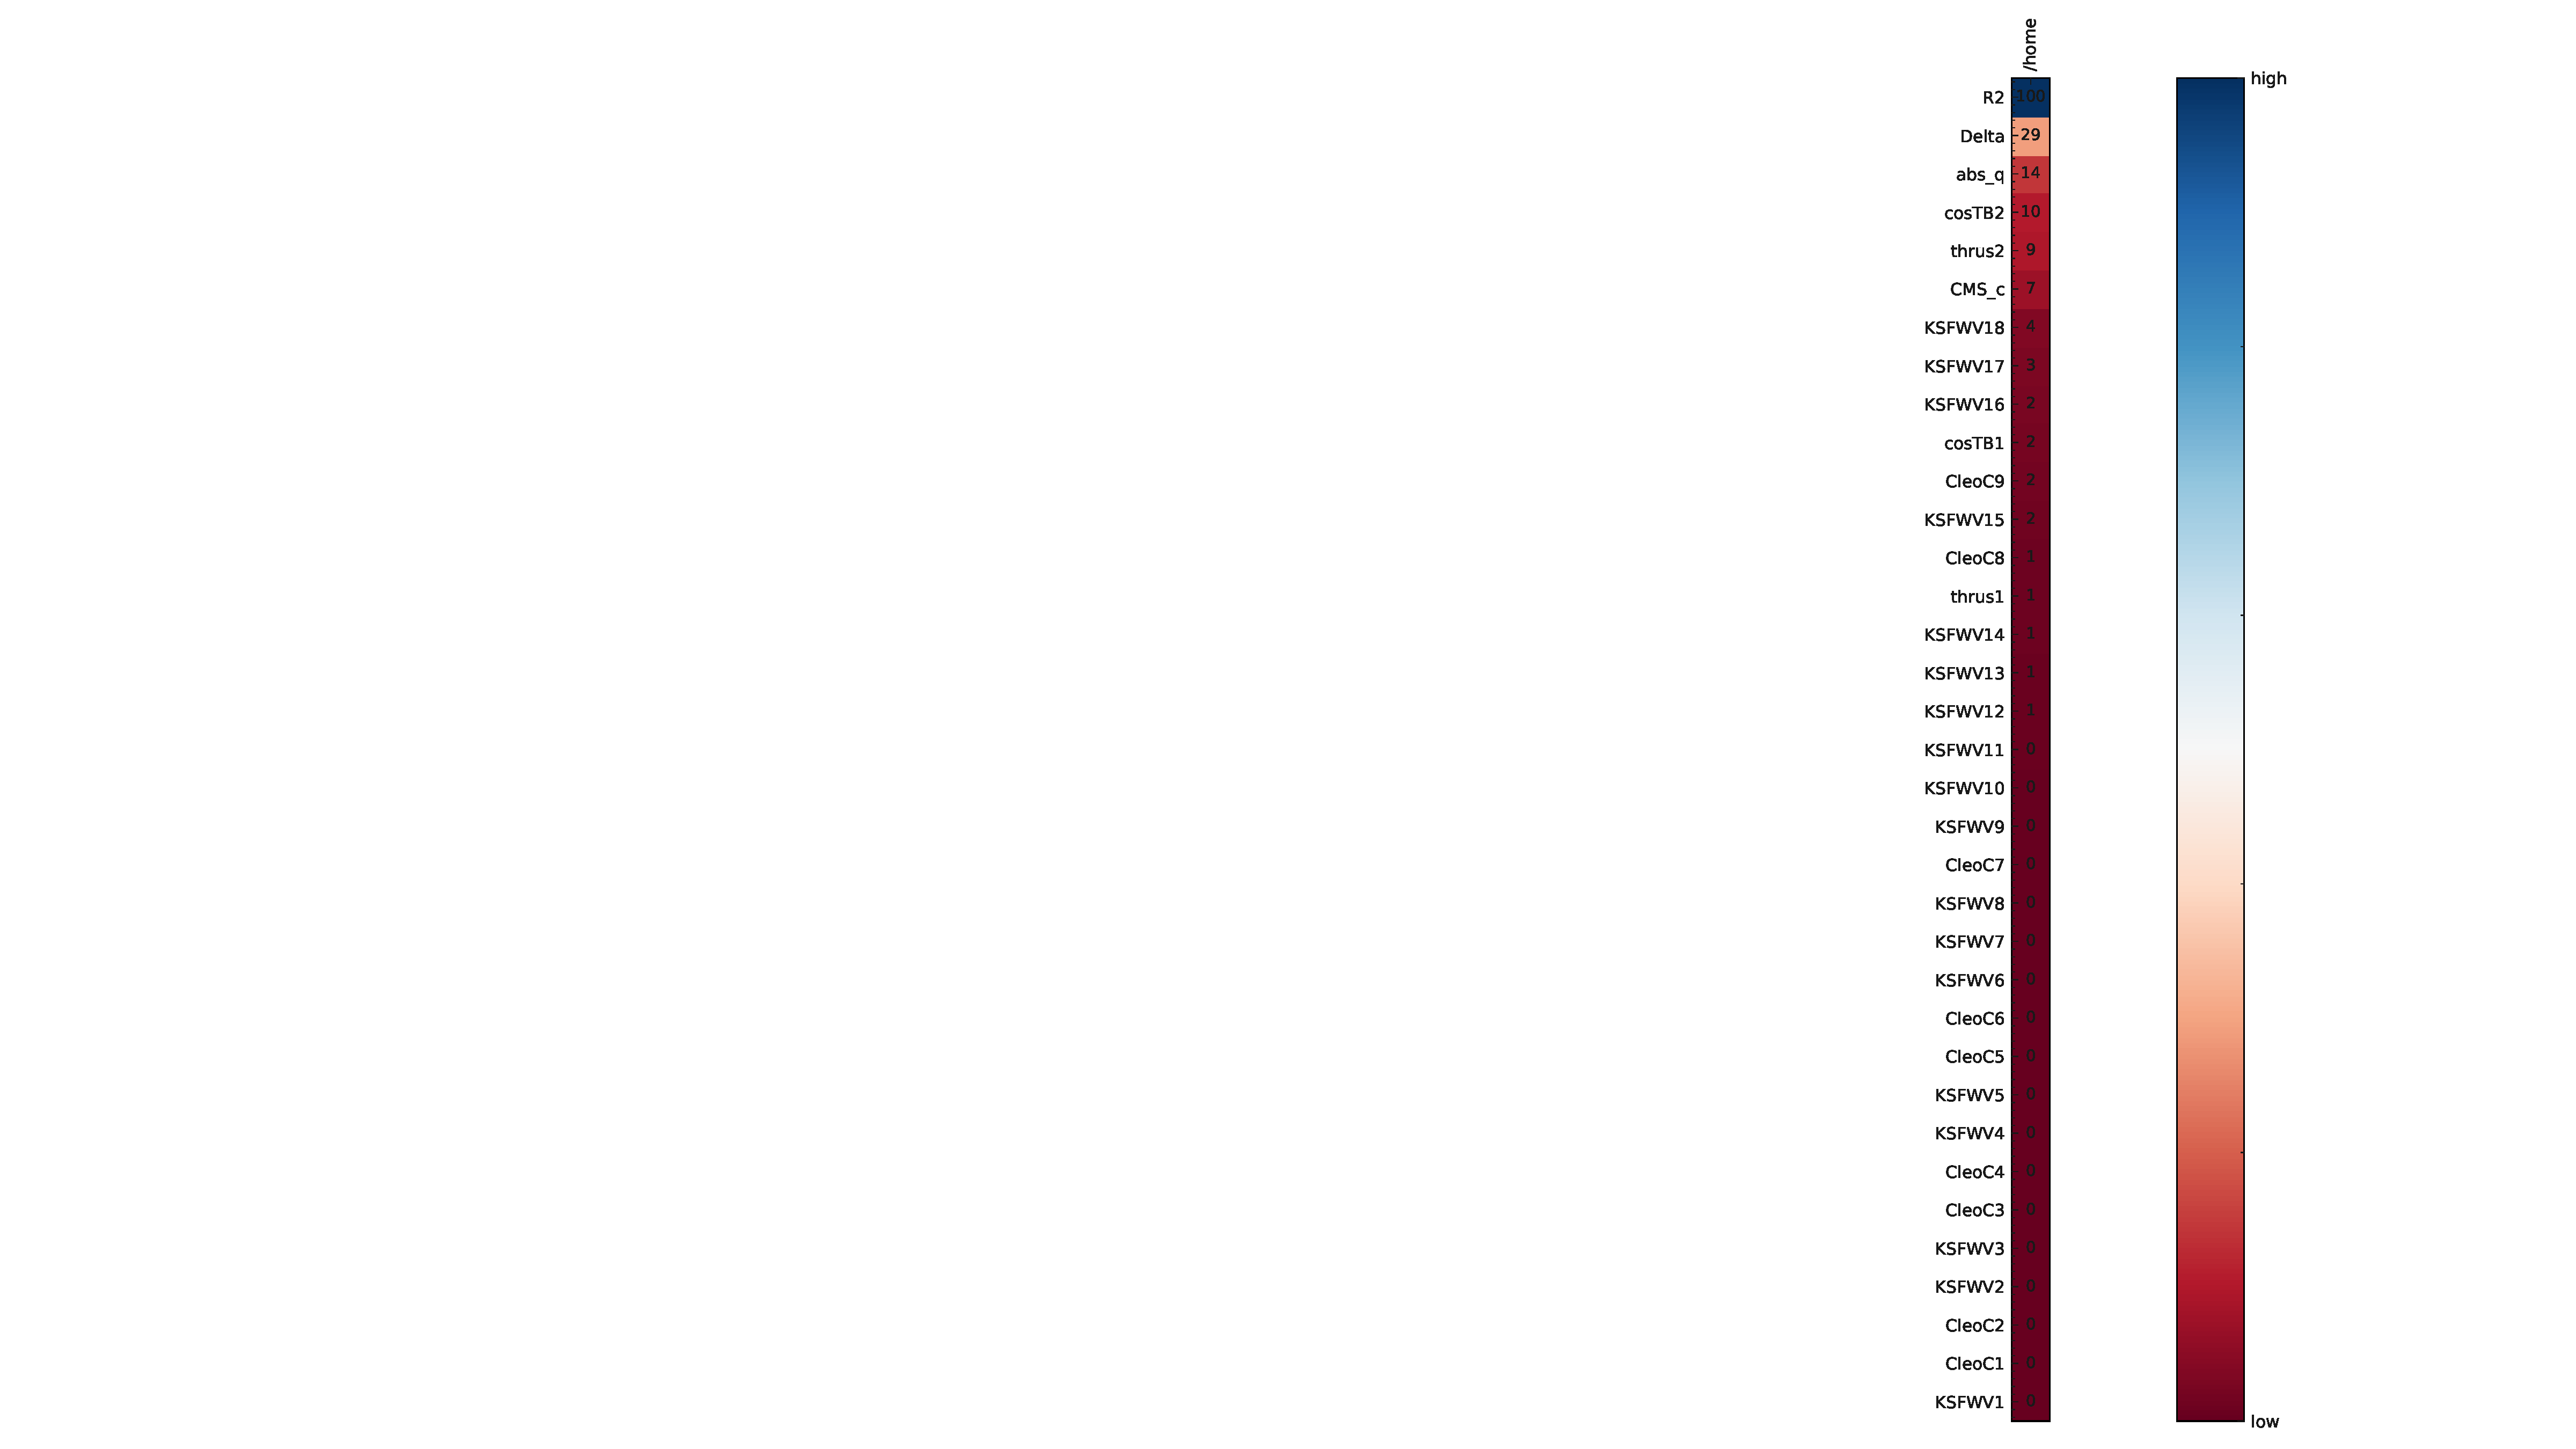
\includegraphics[width=1.0\textwidth]{evaluate_35/importance.pdf}
% 		% \end{figure}
% 	\end{columns}
% \end{frame}
			

% \begin{frame}{ variables}
% \hspace{-1in}
% \includegraphics[width=1.25\textwidth]{evaluate_/importance.pdf}
% 	\vspace{-3.3in}
% 	\begin{columns}
% 		\column{0.7\textwidth}
% 		\begin{figure}
% 			\includegraphics[width=1.0\textwidth]{evaluate_/diagonal_plot_test.pdf}
% 			\includegraphics[width=1.0\textwidth]{evaluate_/overtraining_plot_-6845103939654726996.pdf}
% 		\end{figure}
		
% 		\column{0.3\textwidth}
% 		% \begin{figure}
% 		% 	% \vspace{-0.2 in}
% 		% 	% 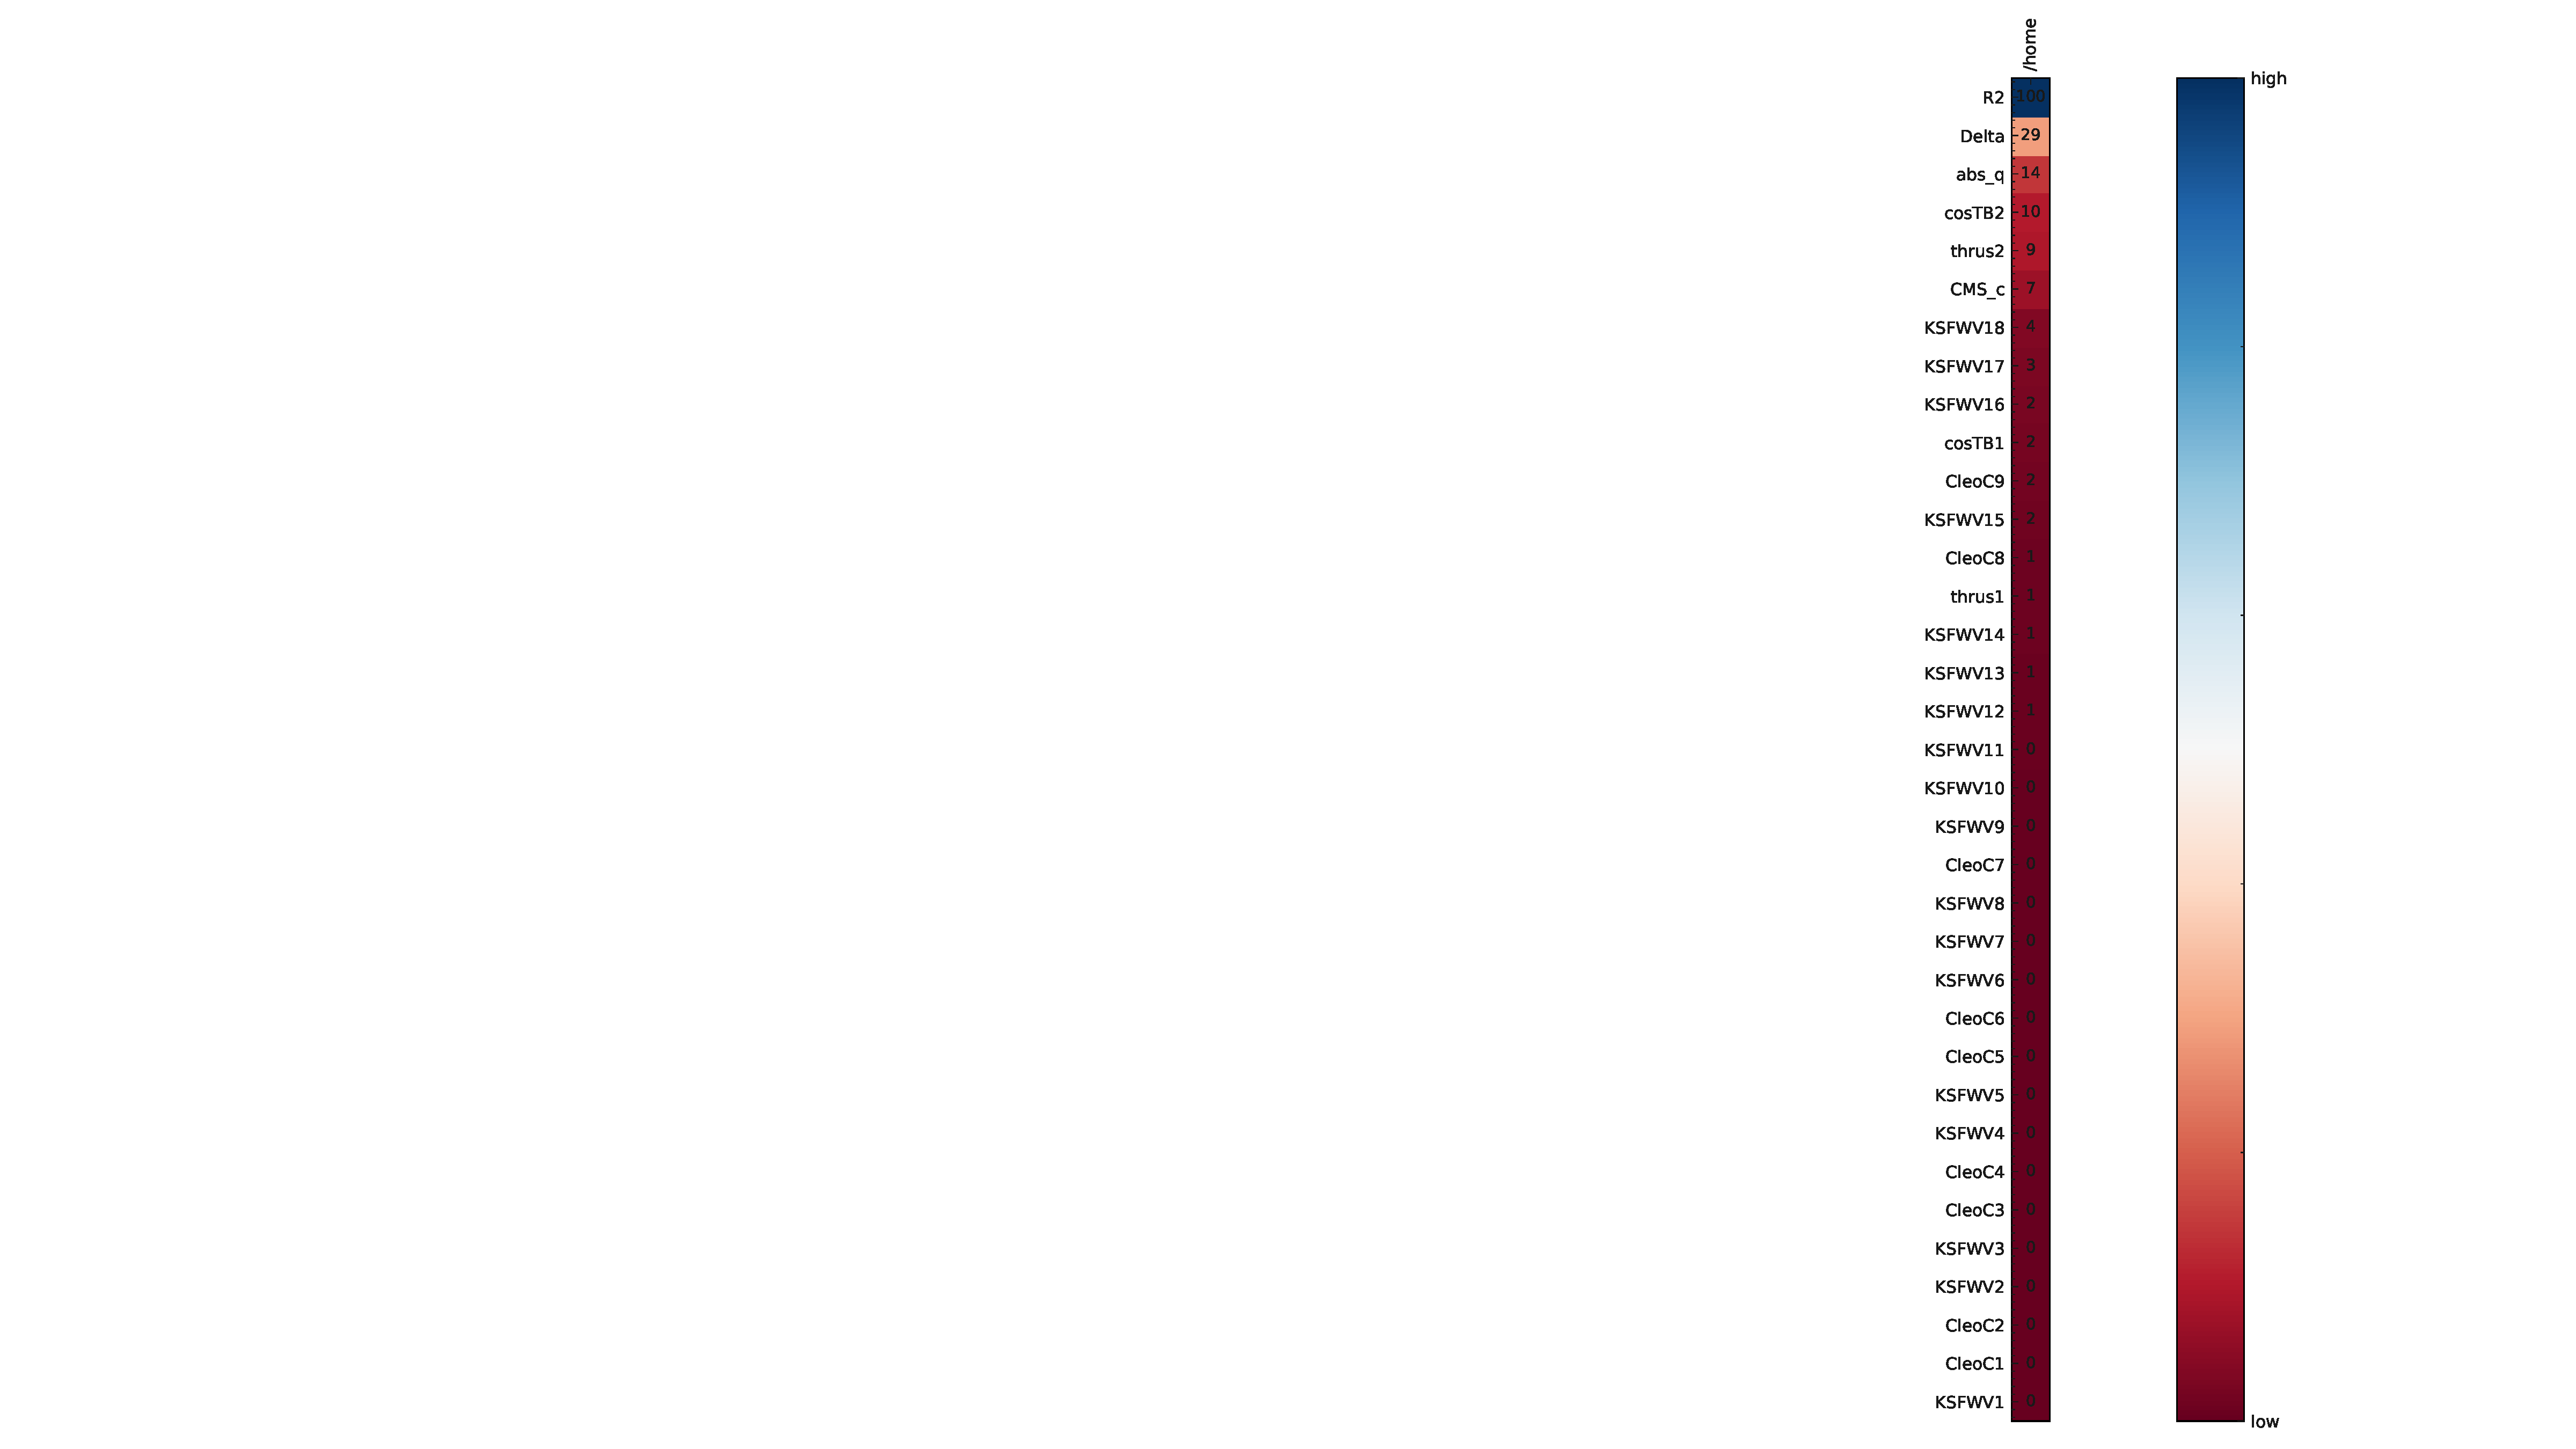
\includegraphics[width=1.0\textwidth]{evaluate_35/importance.pdf}
% 		% \end{figure}
% 	\end{columns}
% \end{frame}
			

\begin{frame}{11 variables}
\hspace{-1in}
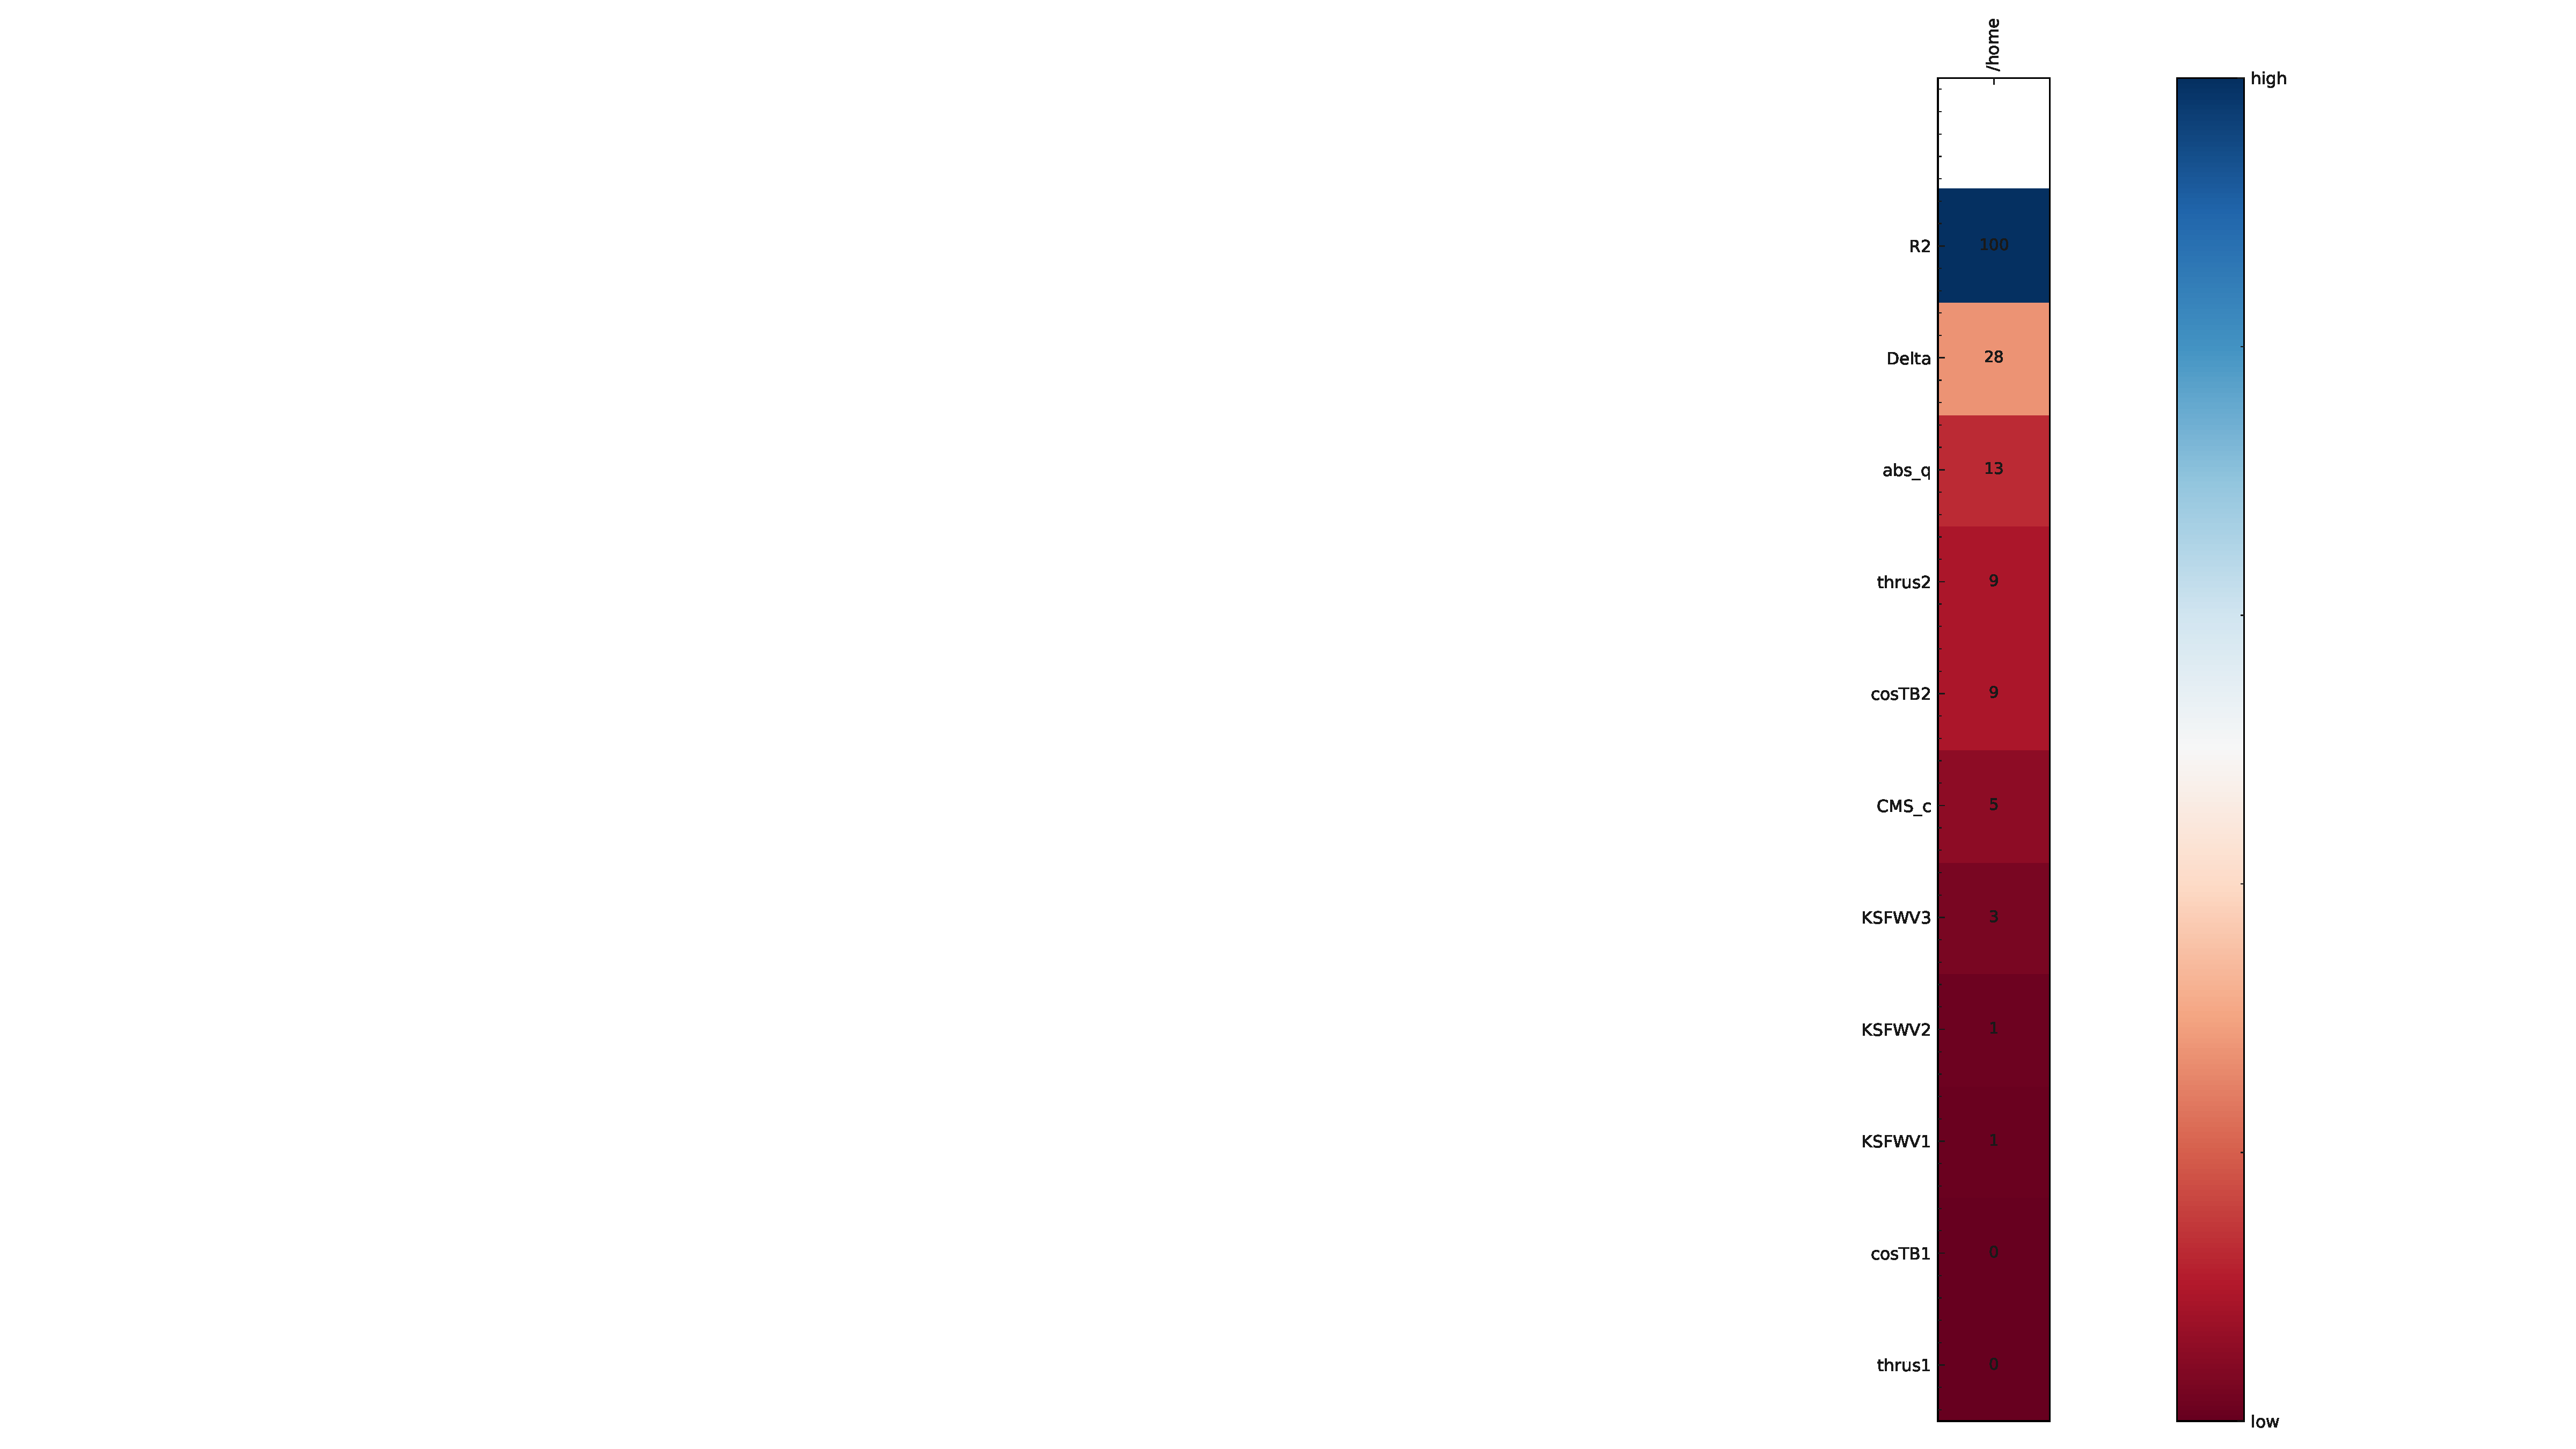
\includegraphics[width=1.25\textwidth]{evaluate_11/importance.pdf}
	\vspace{-3.3in}
	\begin{columns}
		\column{0.7\textwidth}
		\begin{figure}
			\includegraphics[width=1.0\textwidth]{evaluate_11/diagonal_plot_test.pdf}
			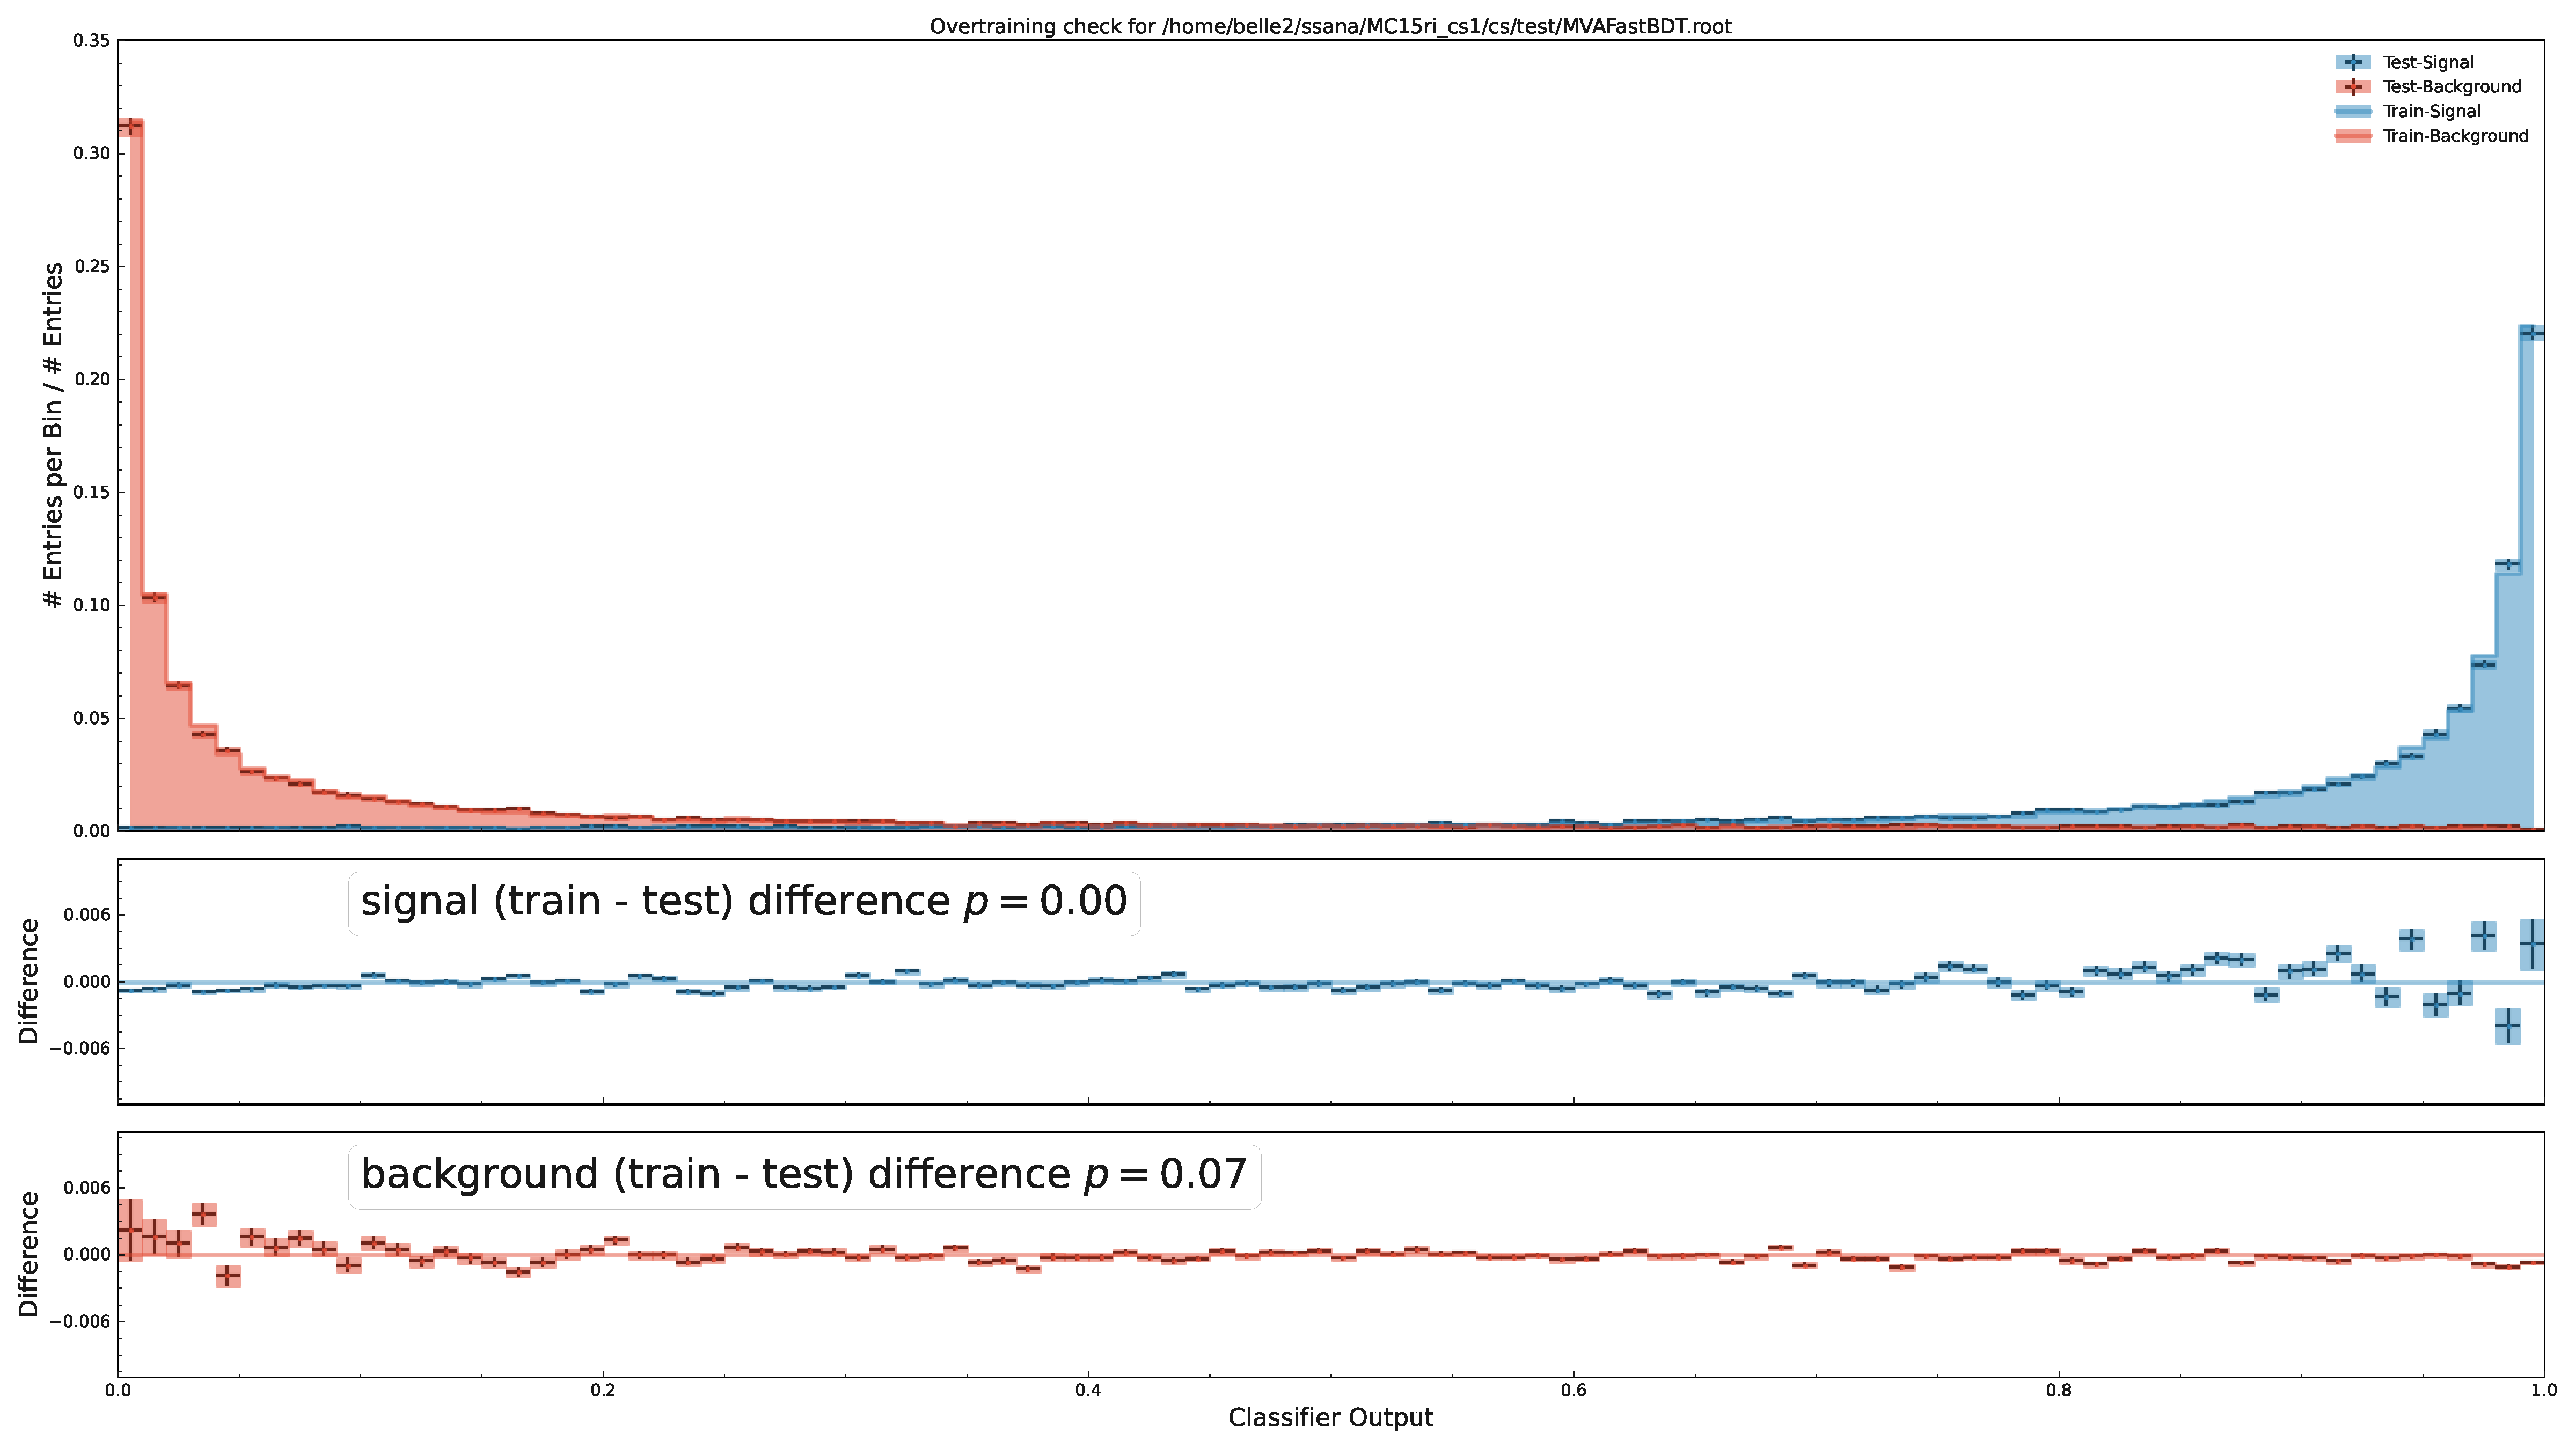
\includegraphics[width=1.0\textwidth]{evaluate_11/overtraining_plot_-2246559386340646363.pdf}
		\end{figure}
		
		\column{0.3\textwidth}
		% \begin{figure}
		% 	% \vspace{-0.2 in}
		% 	% 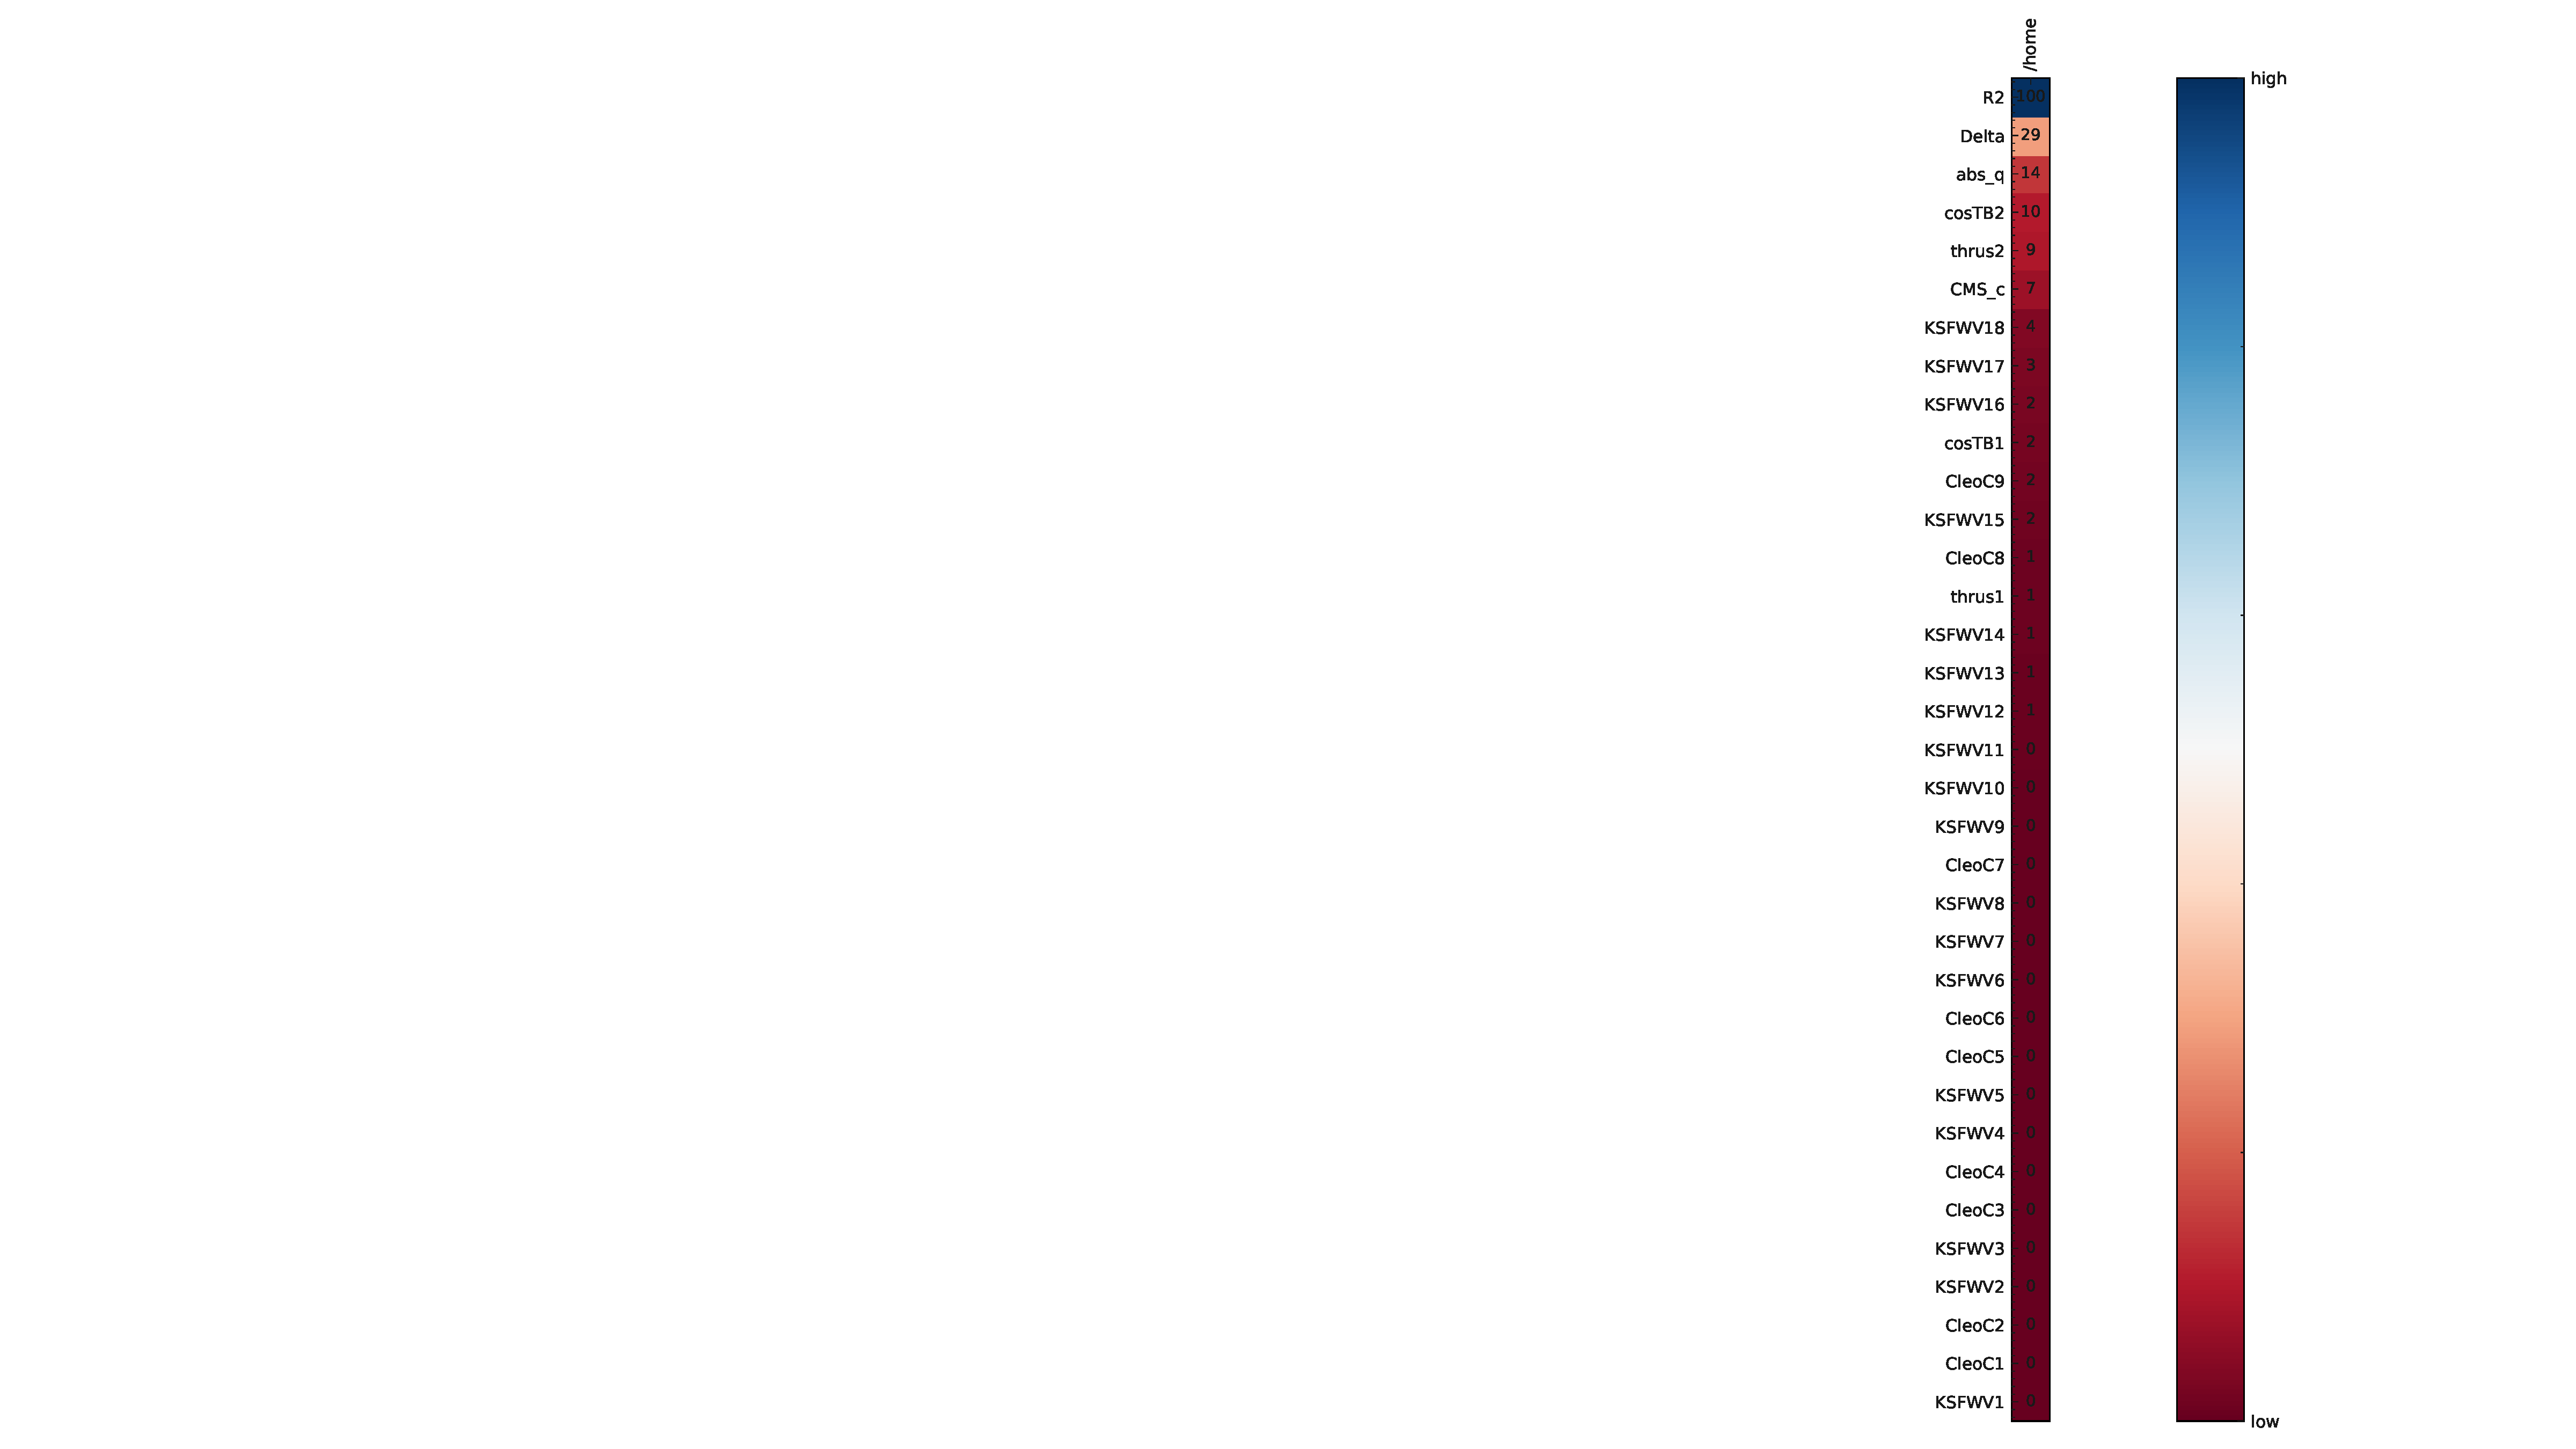
\includegraphics[width=1.0\textwidth]{evaluate_35/importance.pdf}
		% \end{figure}
	\end{columns}
\end{frame}

\begin{frame}{14 variables}
\hspace{-1in}
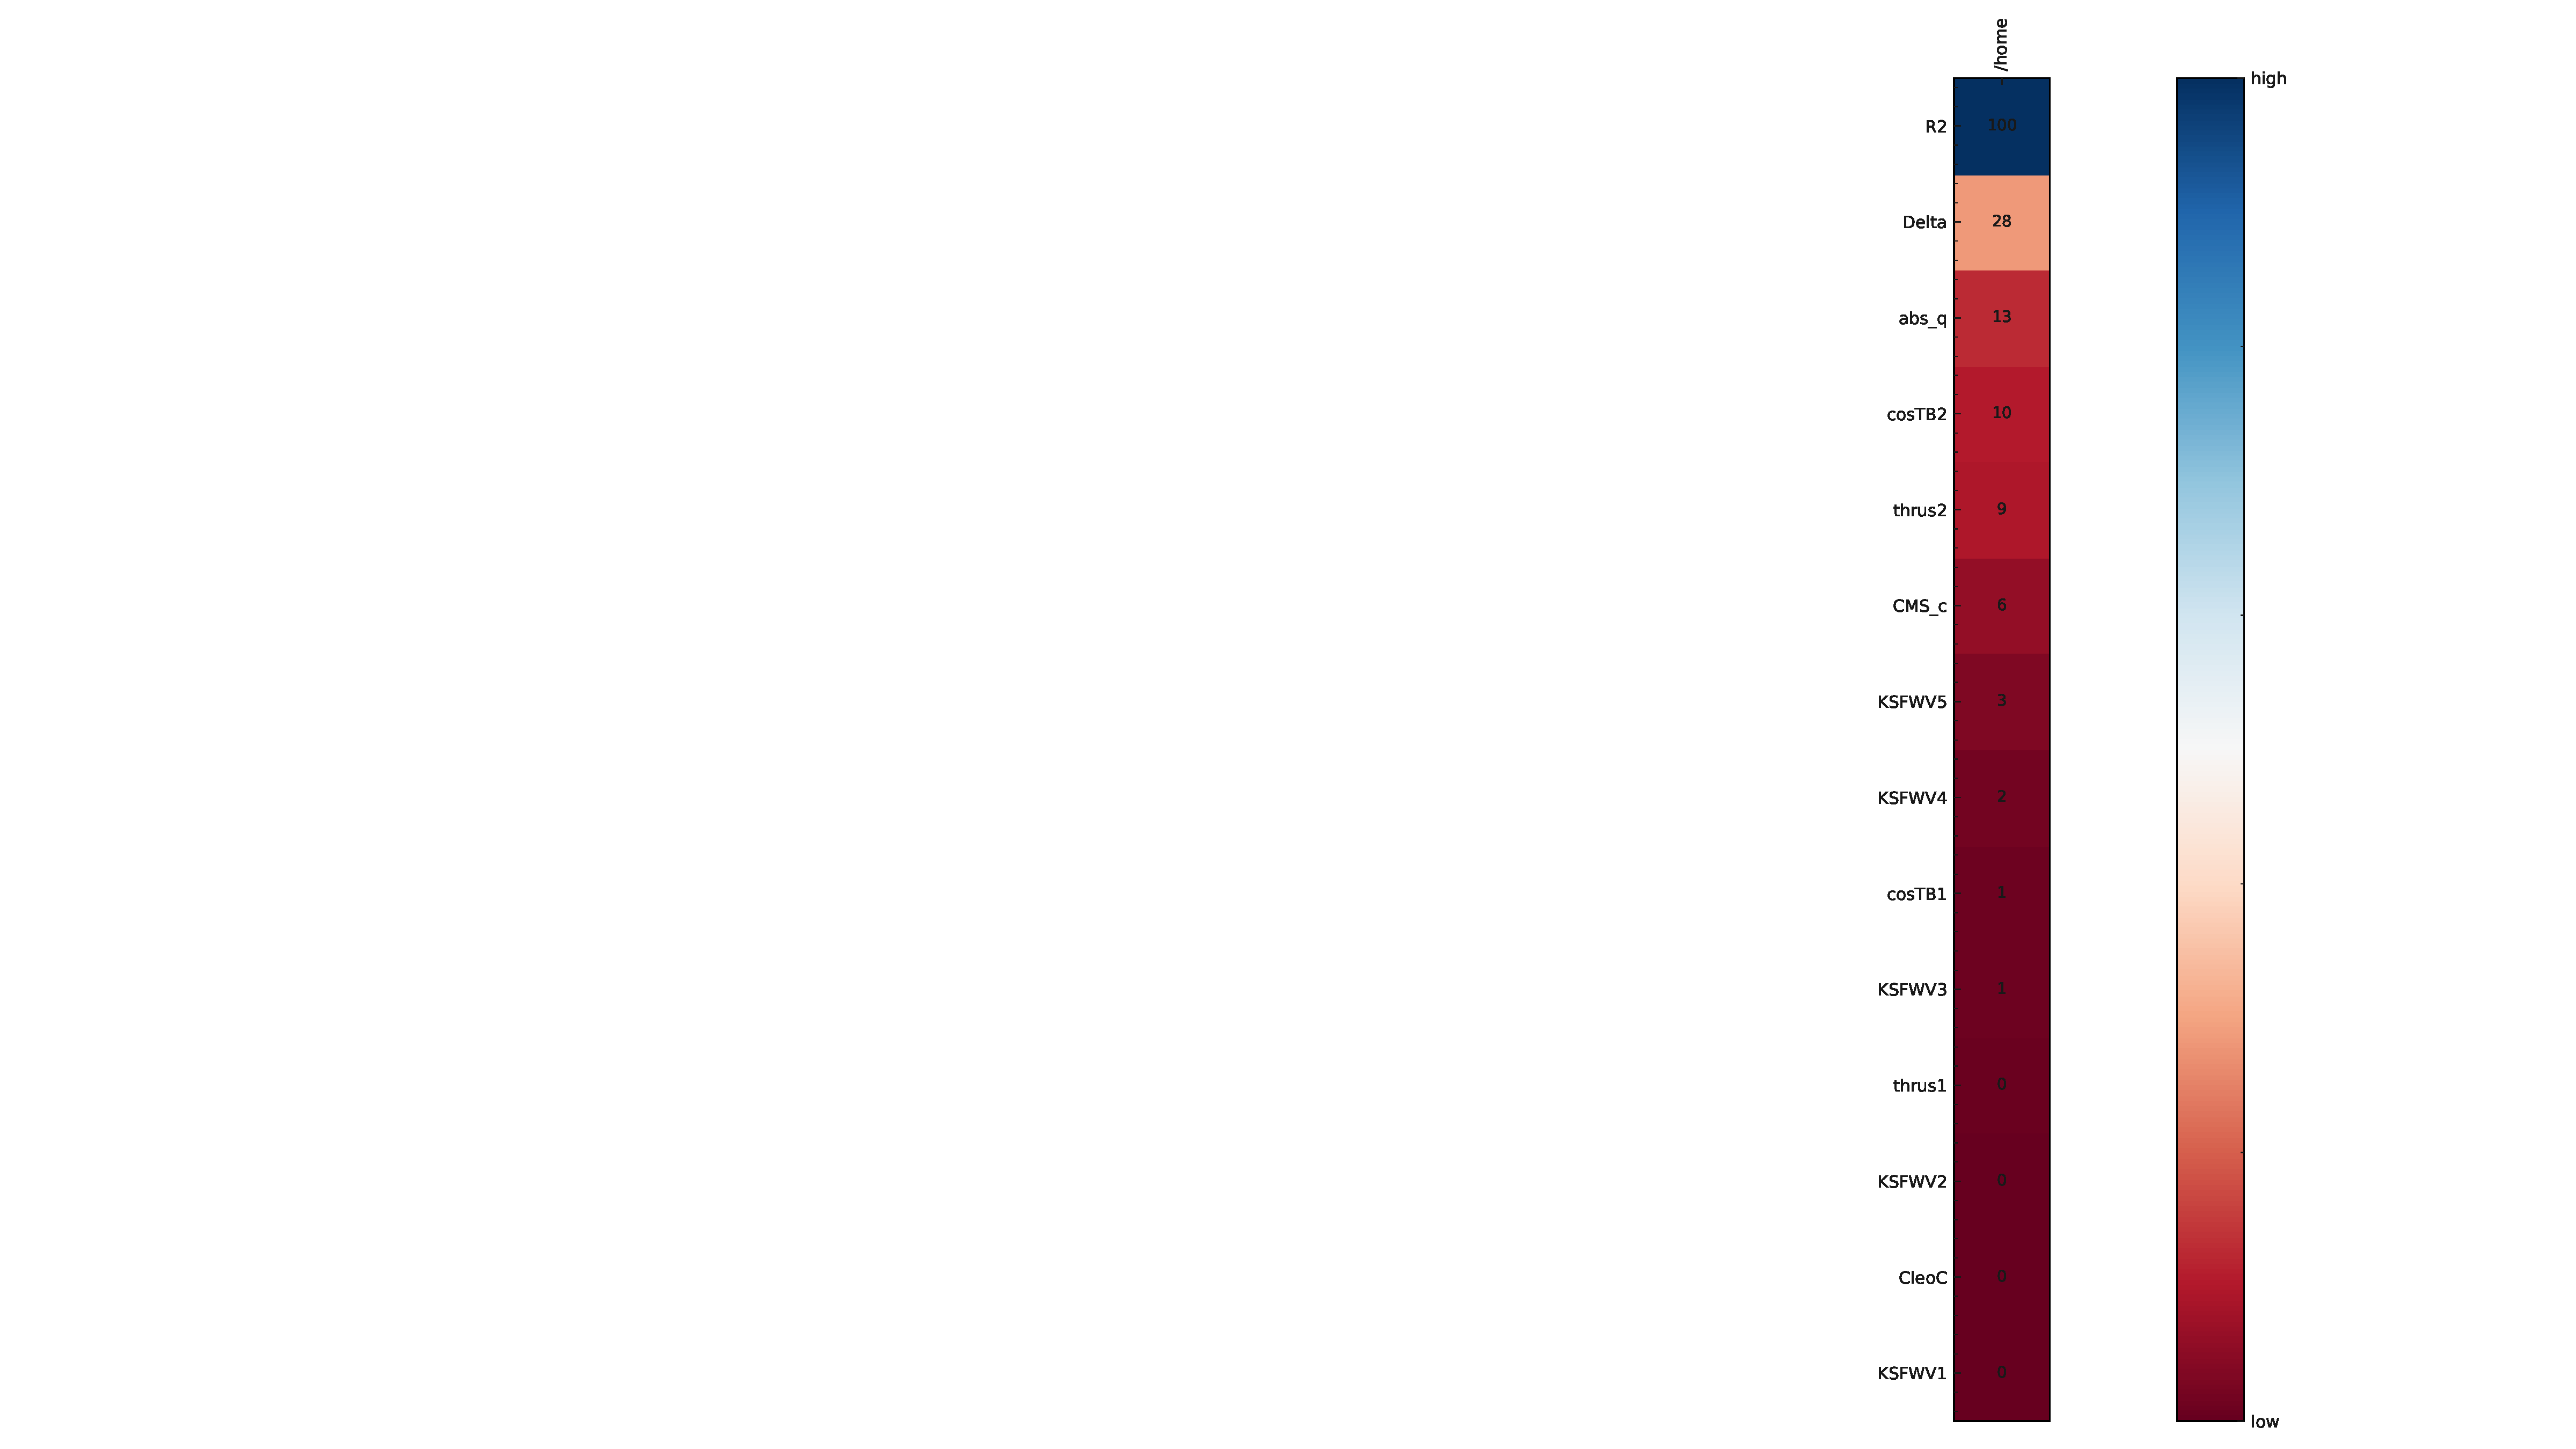
\includegraphics[width=1.25\textwidth]{evaluate_14/importance.pdf}
	\vspace{-3.3in}
	\begin{columns}
		\column{0.7\textwidth}
		\begin{figure}
			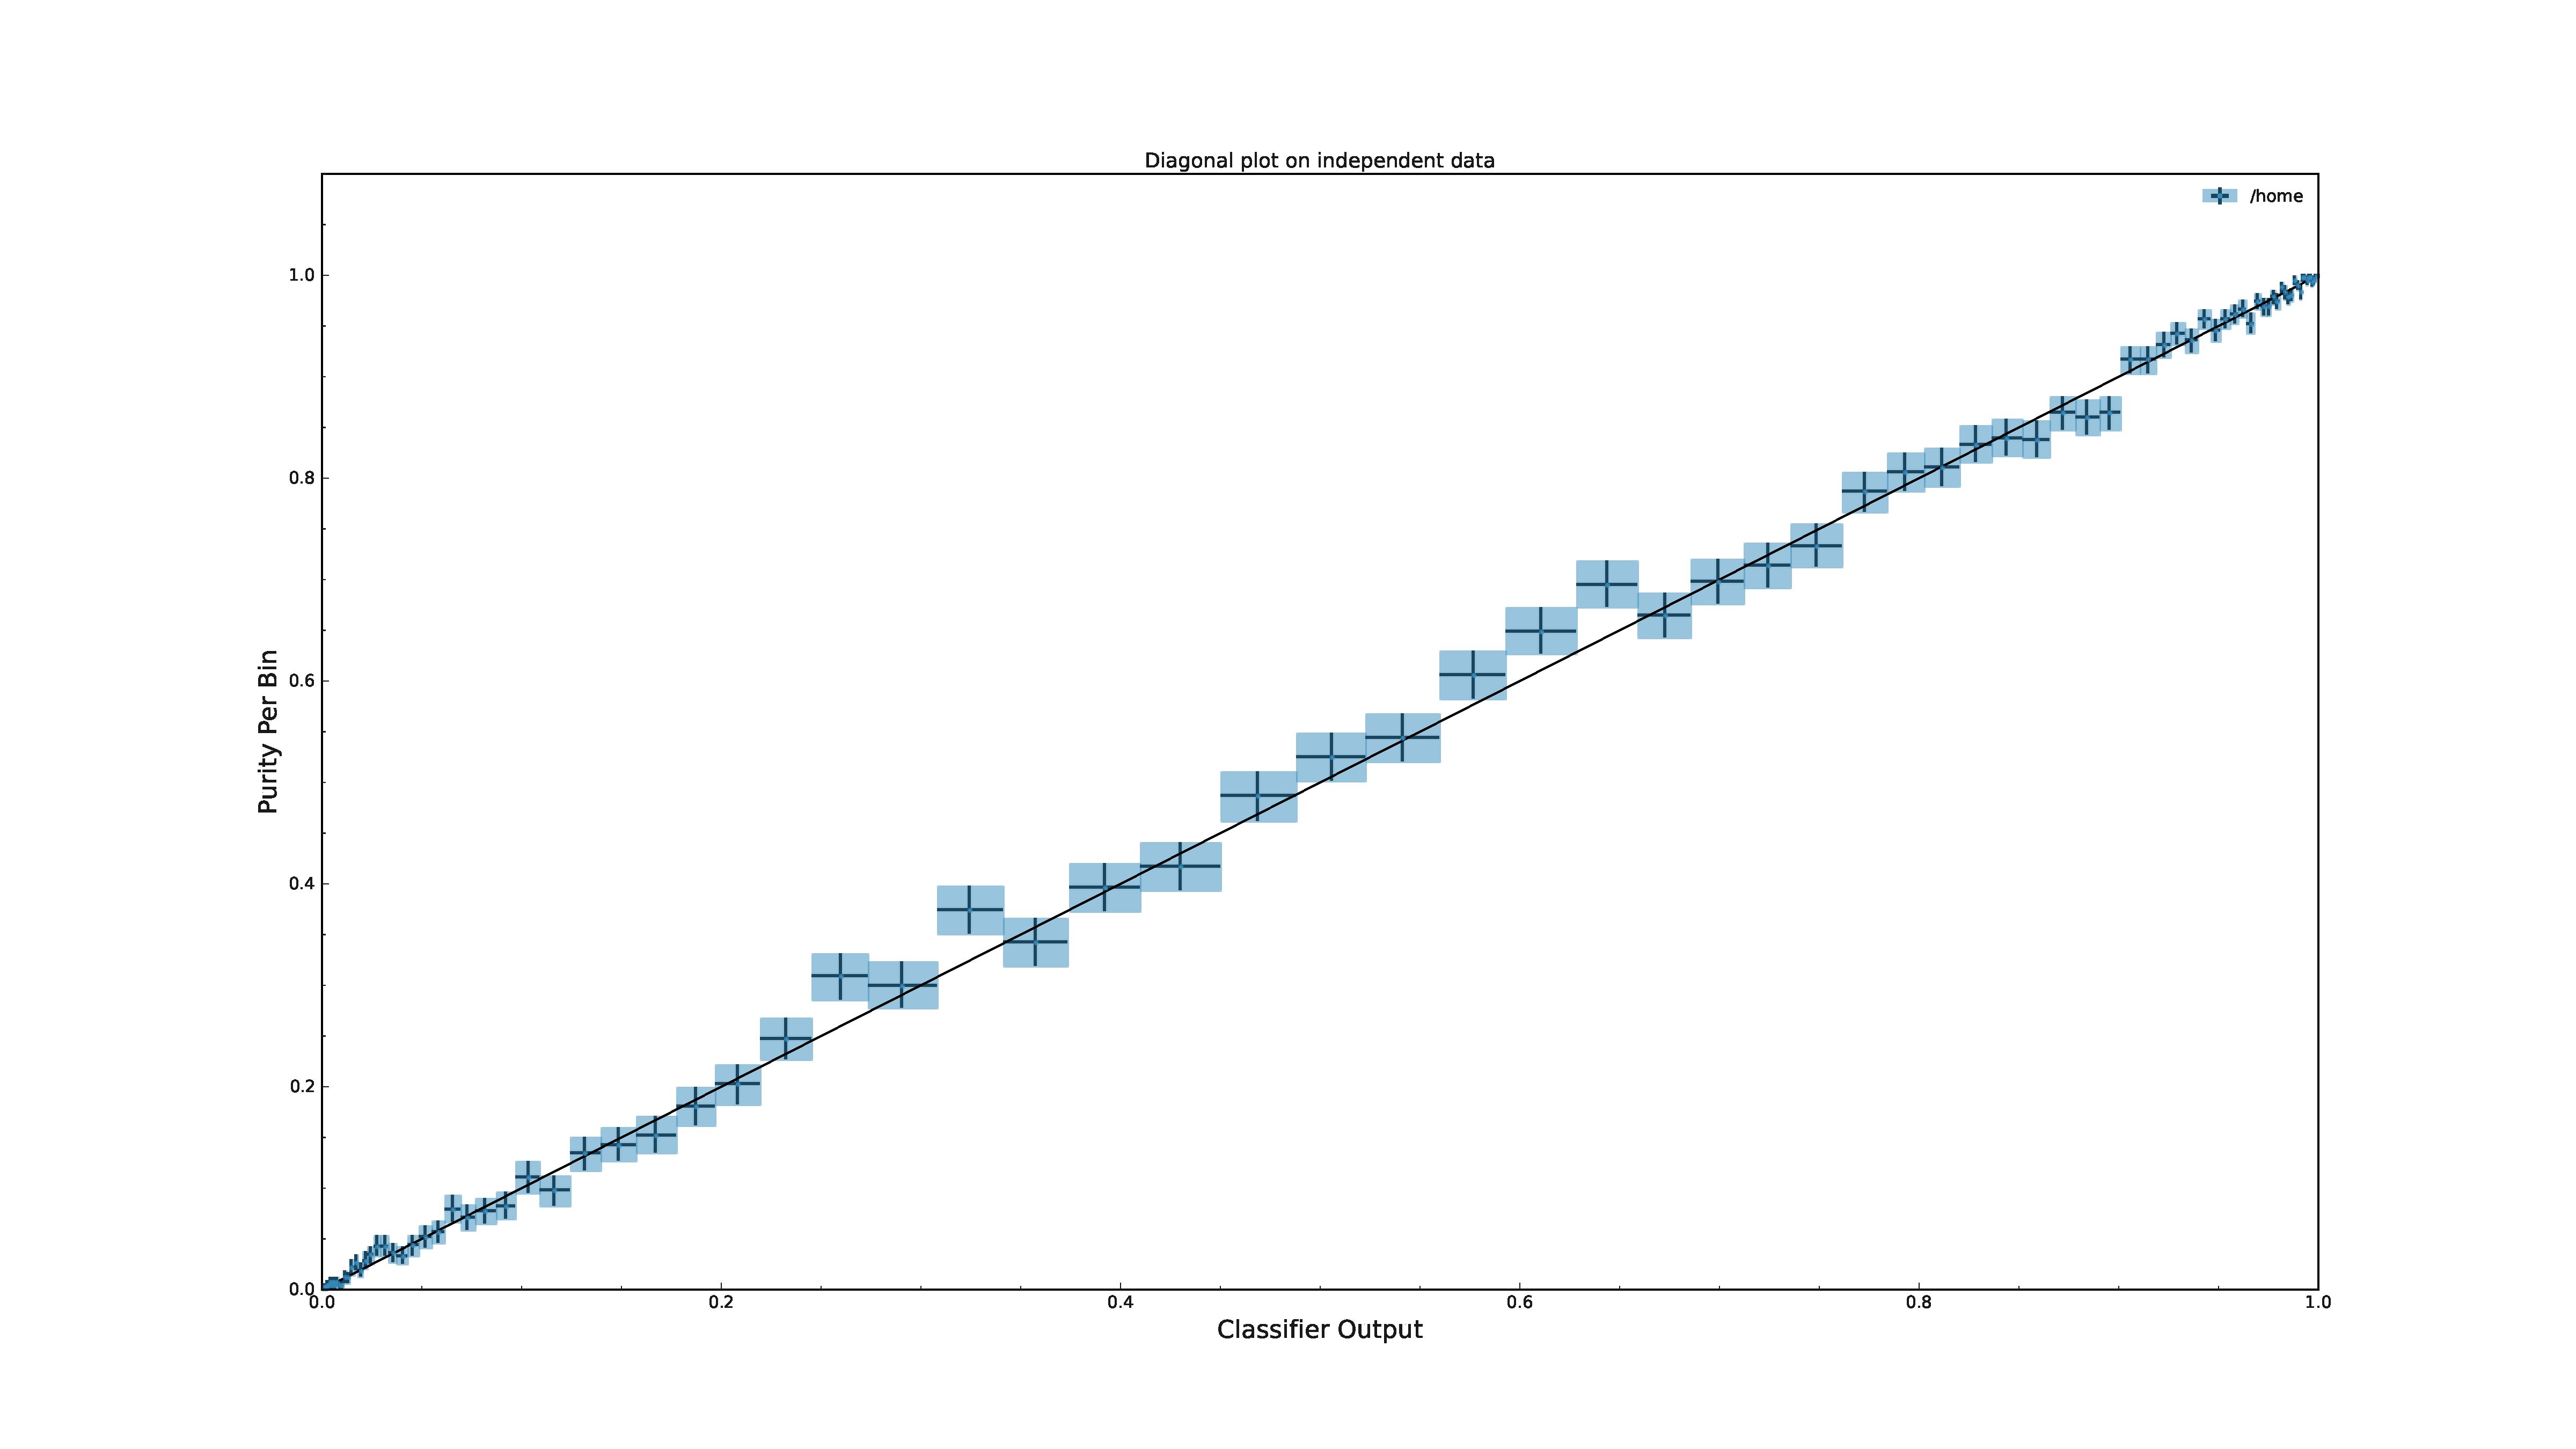
\includegraphics[width=1.0\textwidth]{evaluate_14/diagonal_plot_test.pdf}
			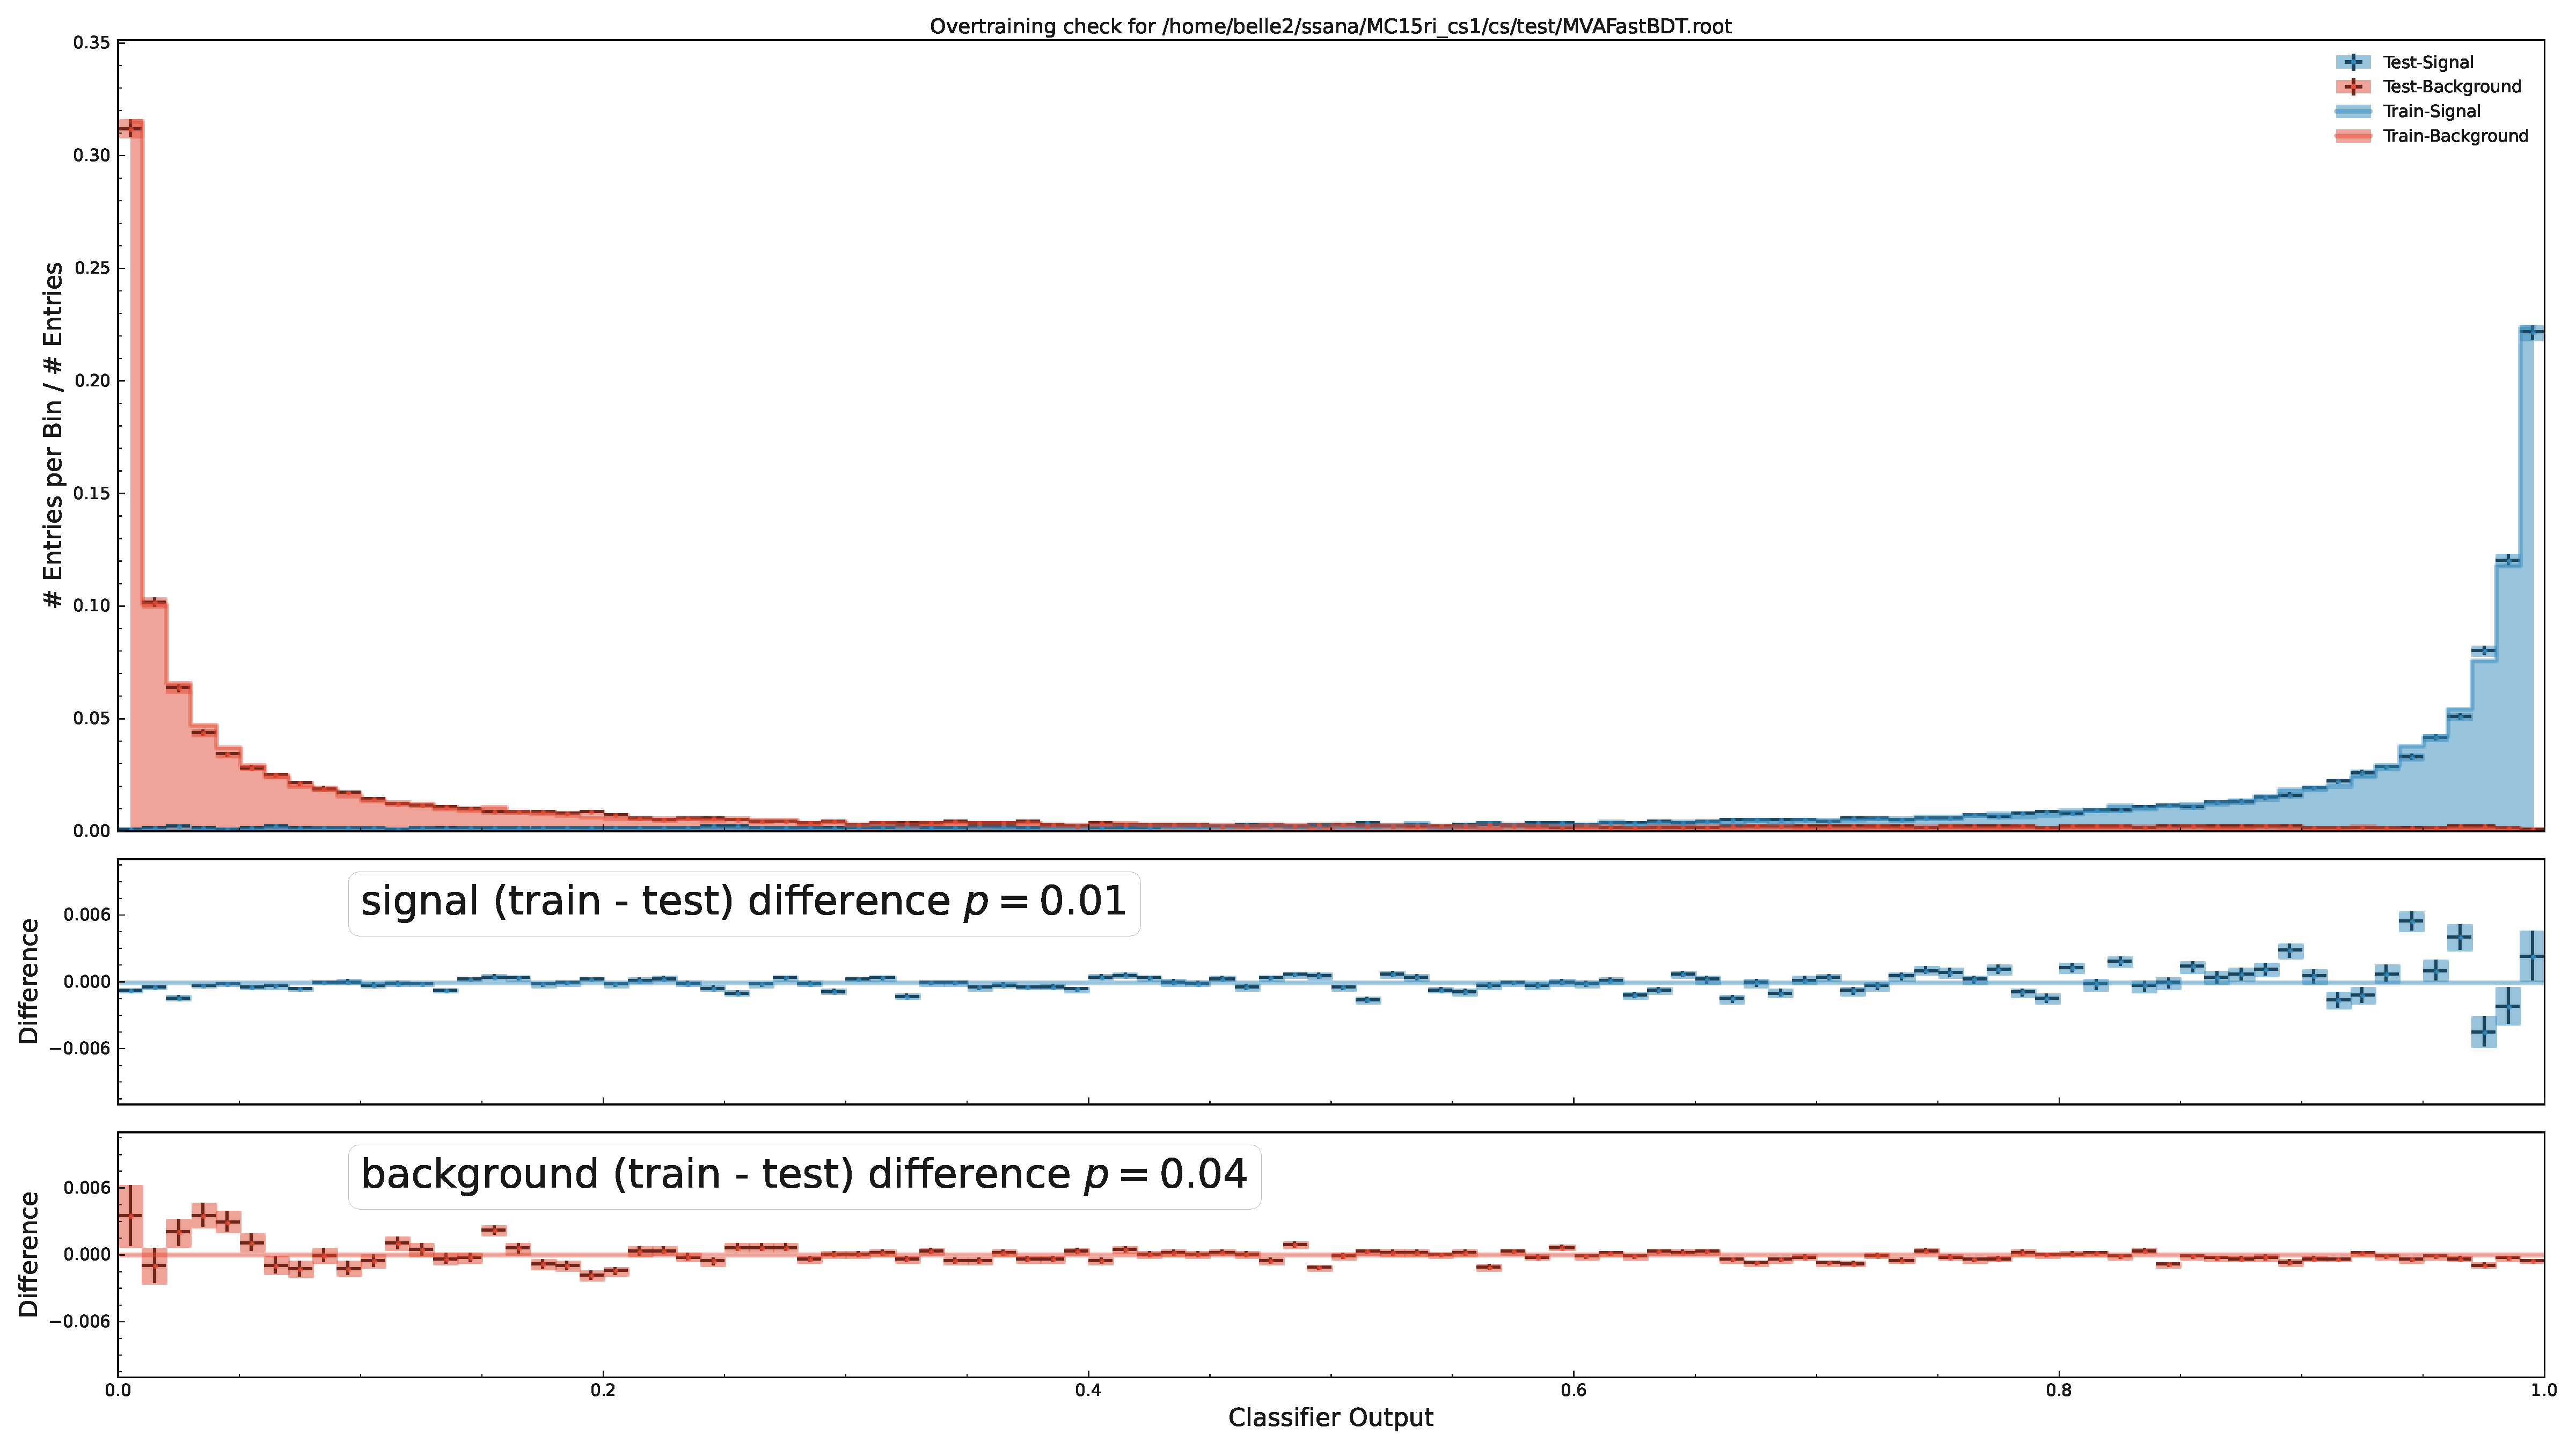
\includegraphics[width=1.0\textwidth]{evaluate_14/overtraining_plot_-6962044671939454446.pdf}
		\end{figure}
		
		\column{0.3\textwidth}
		% \begin{figure}
		% 	% \vspace{-0.2 in}
		% 	% 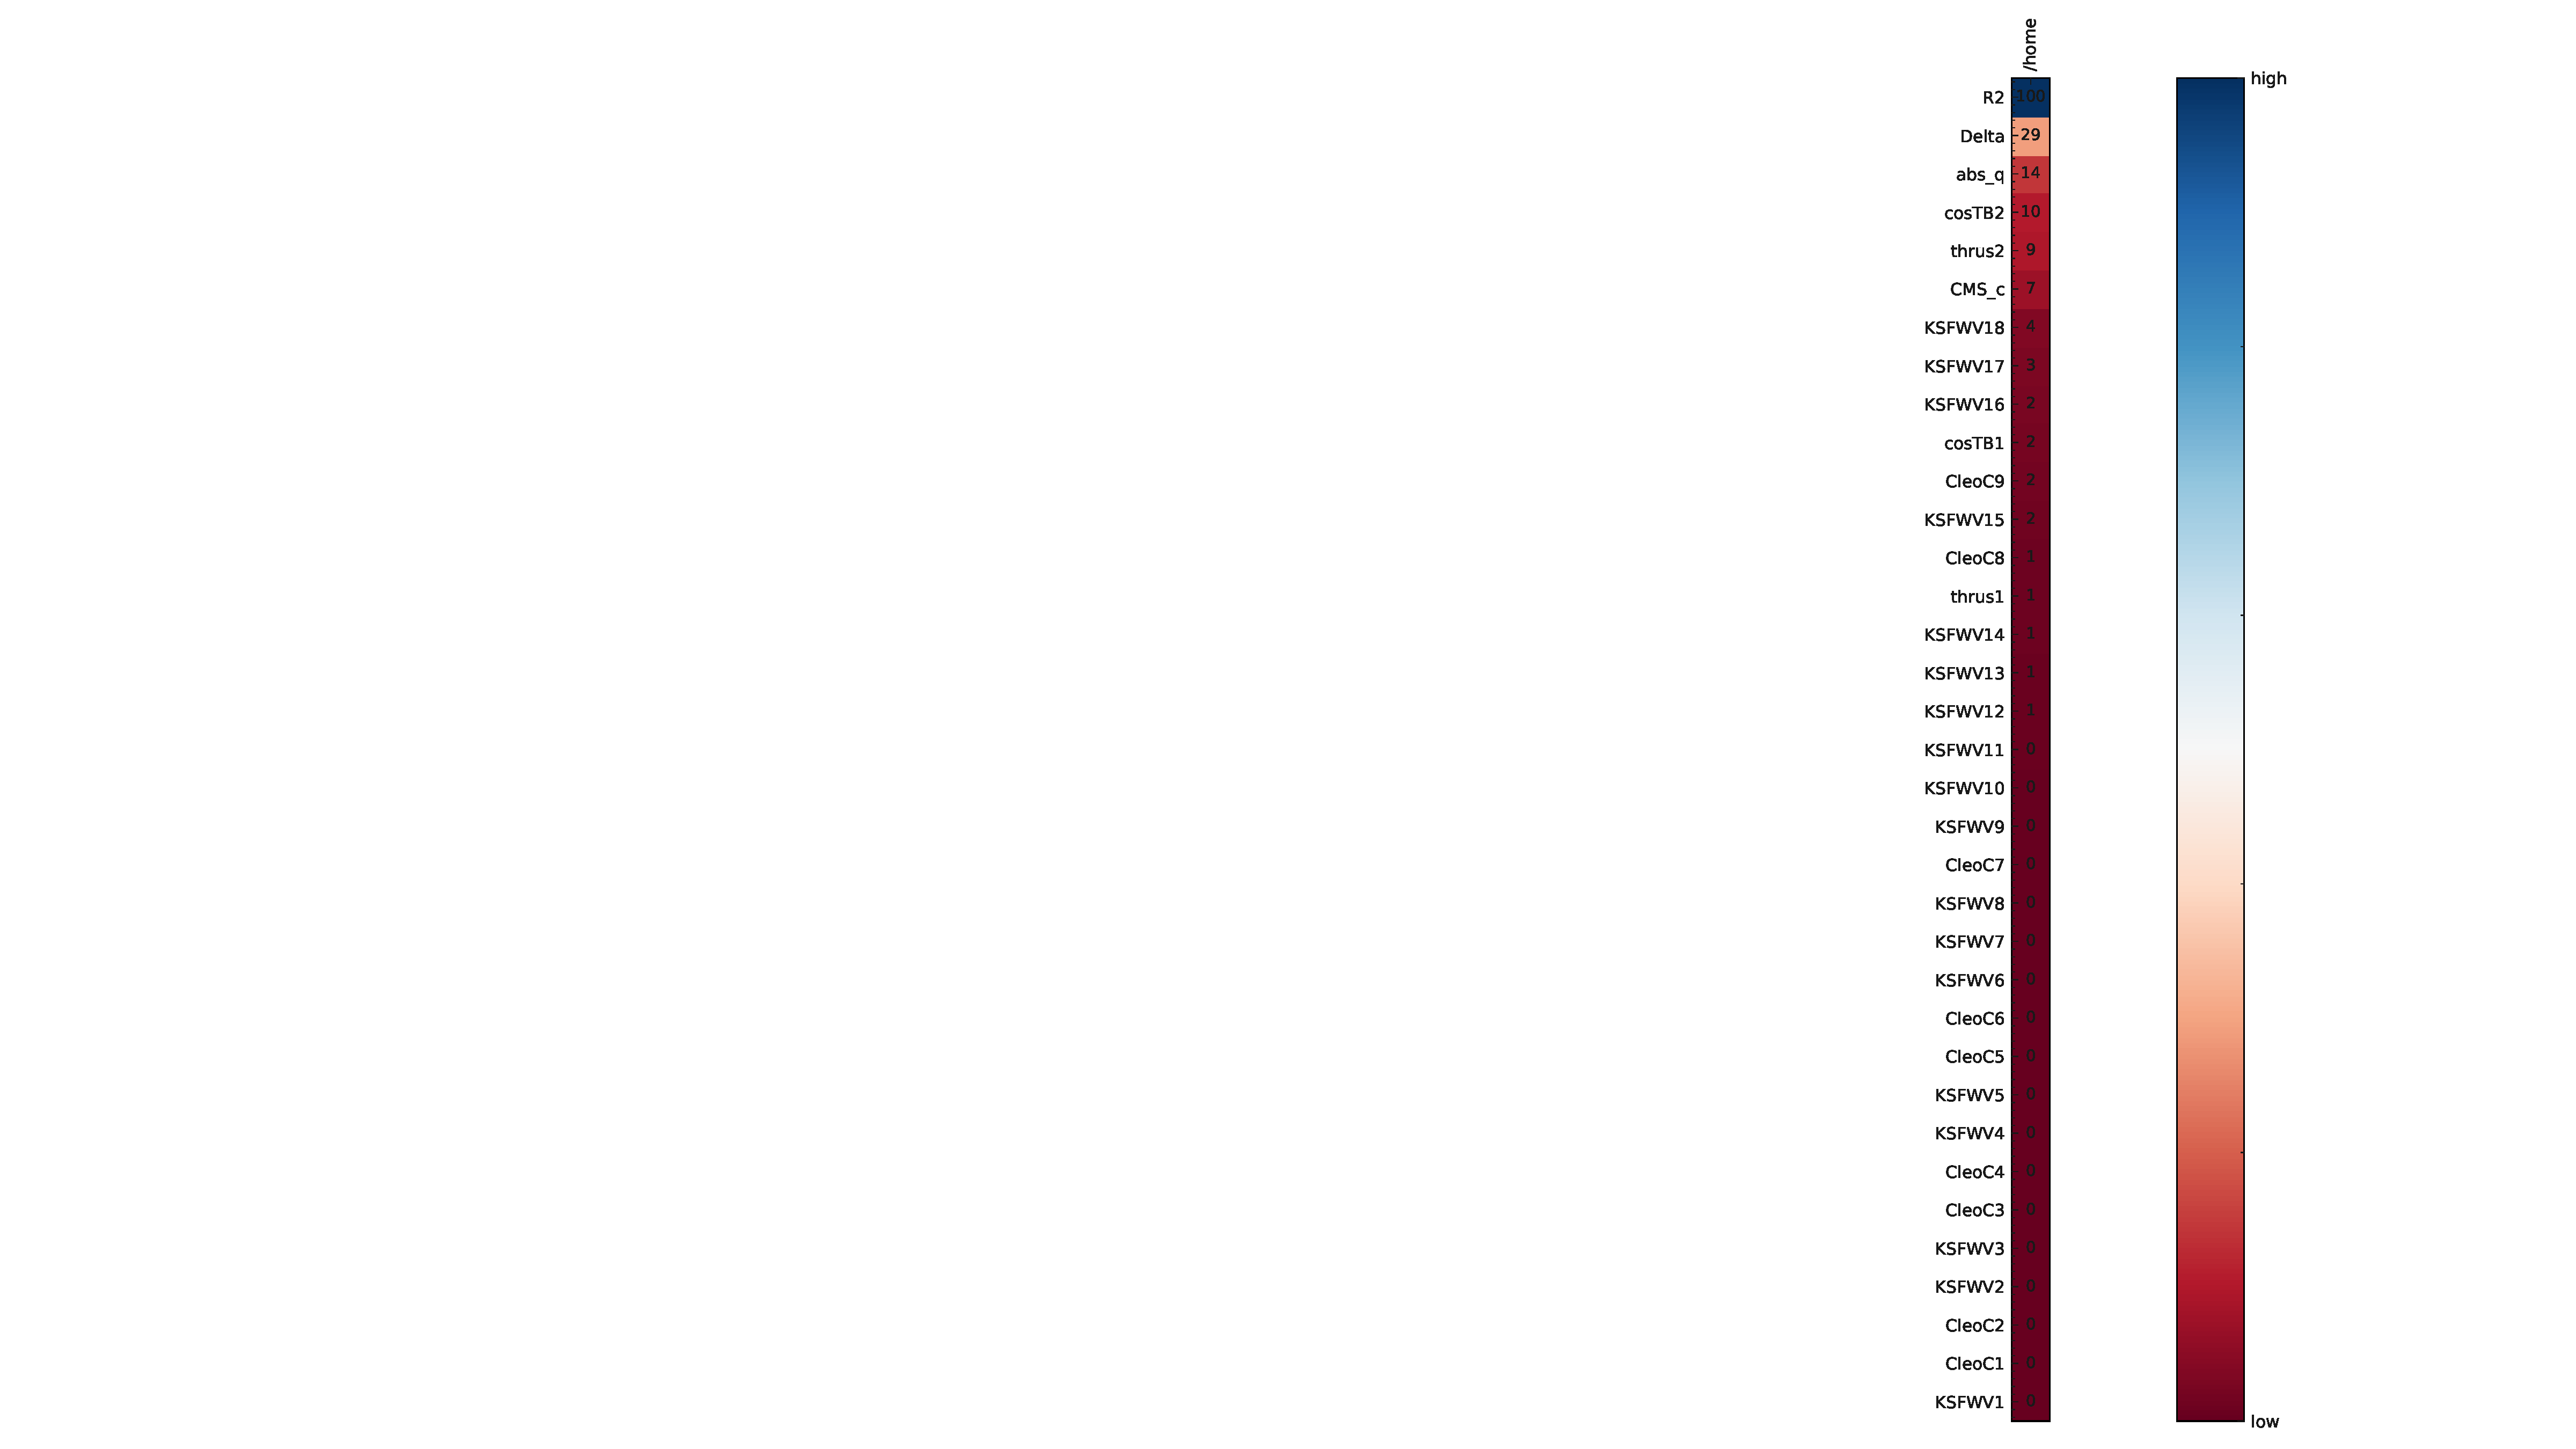
\includegraphics[width=1.0\textwidth]{evaluate_35/importance.pdf}
		% \end{figure}
	\end{columns}
\end{frame}
\begin{frame}{17 variables}
\hspace{-1in}
\includegraphics[width=1.25\textwidth]{evaluate_17/importance.pdf}
	\vspace{-3.3in}
	\begin{columns}
		\column{0.7\textwidth}
		\begin{figure}
			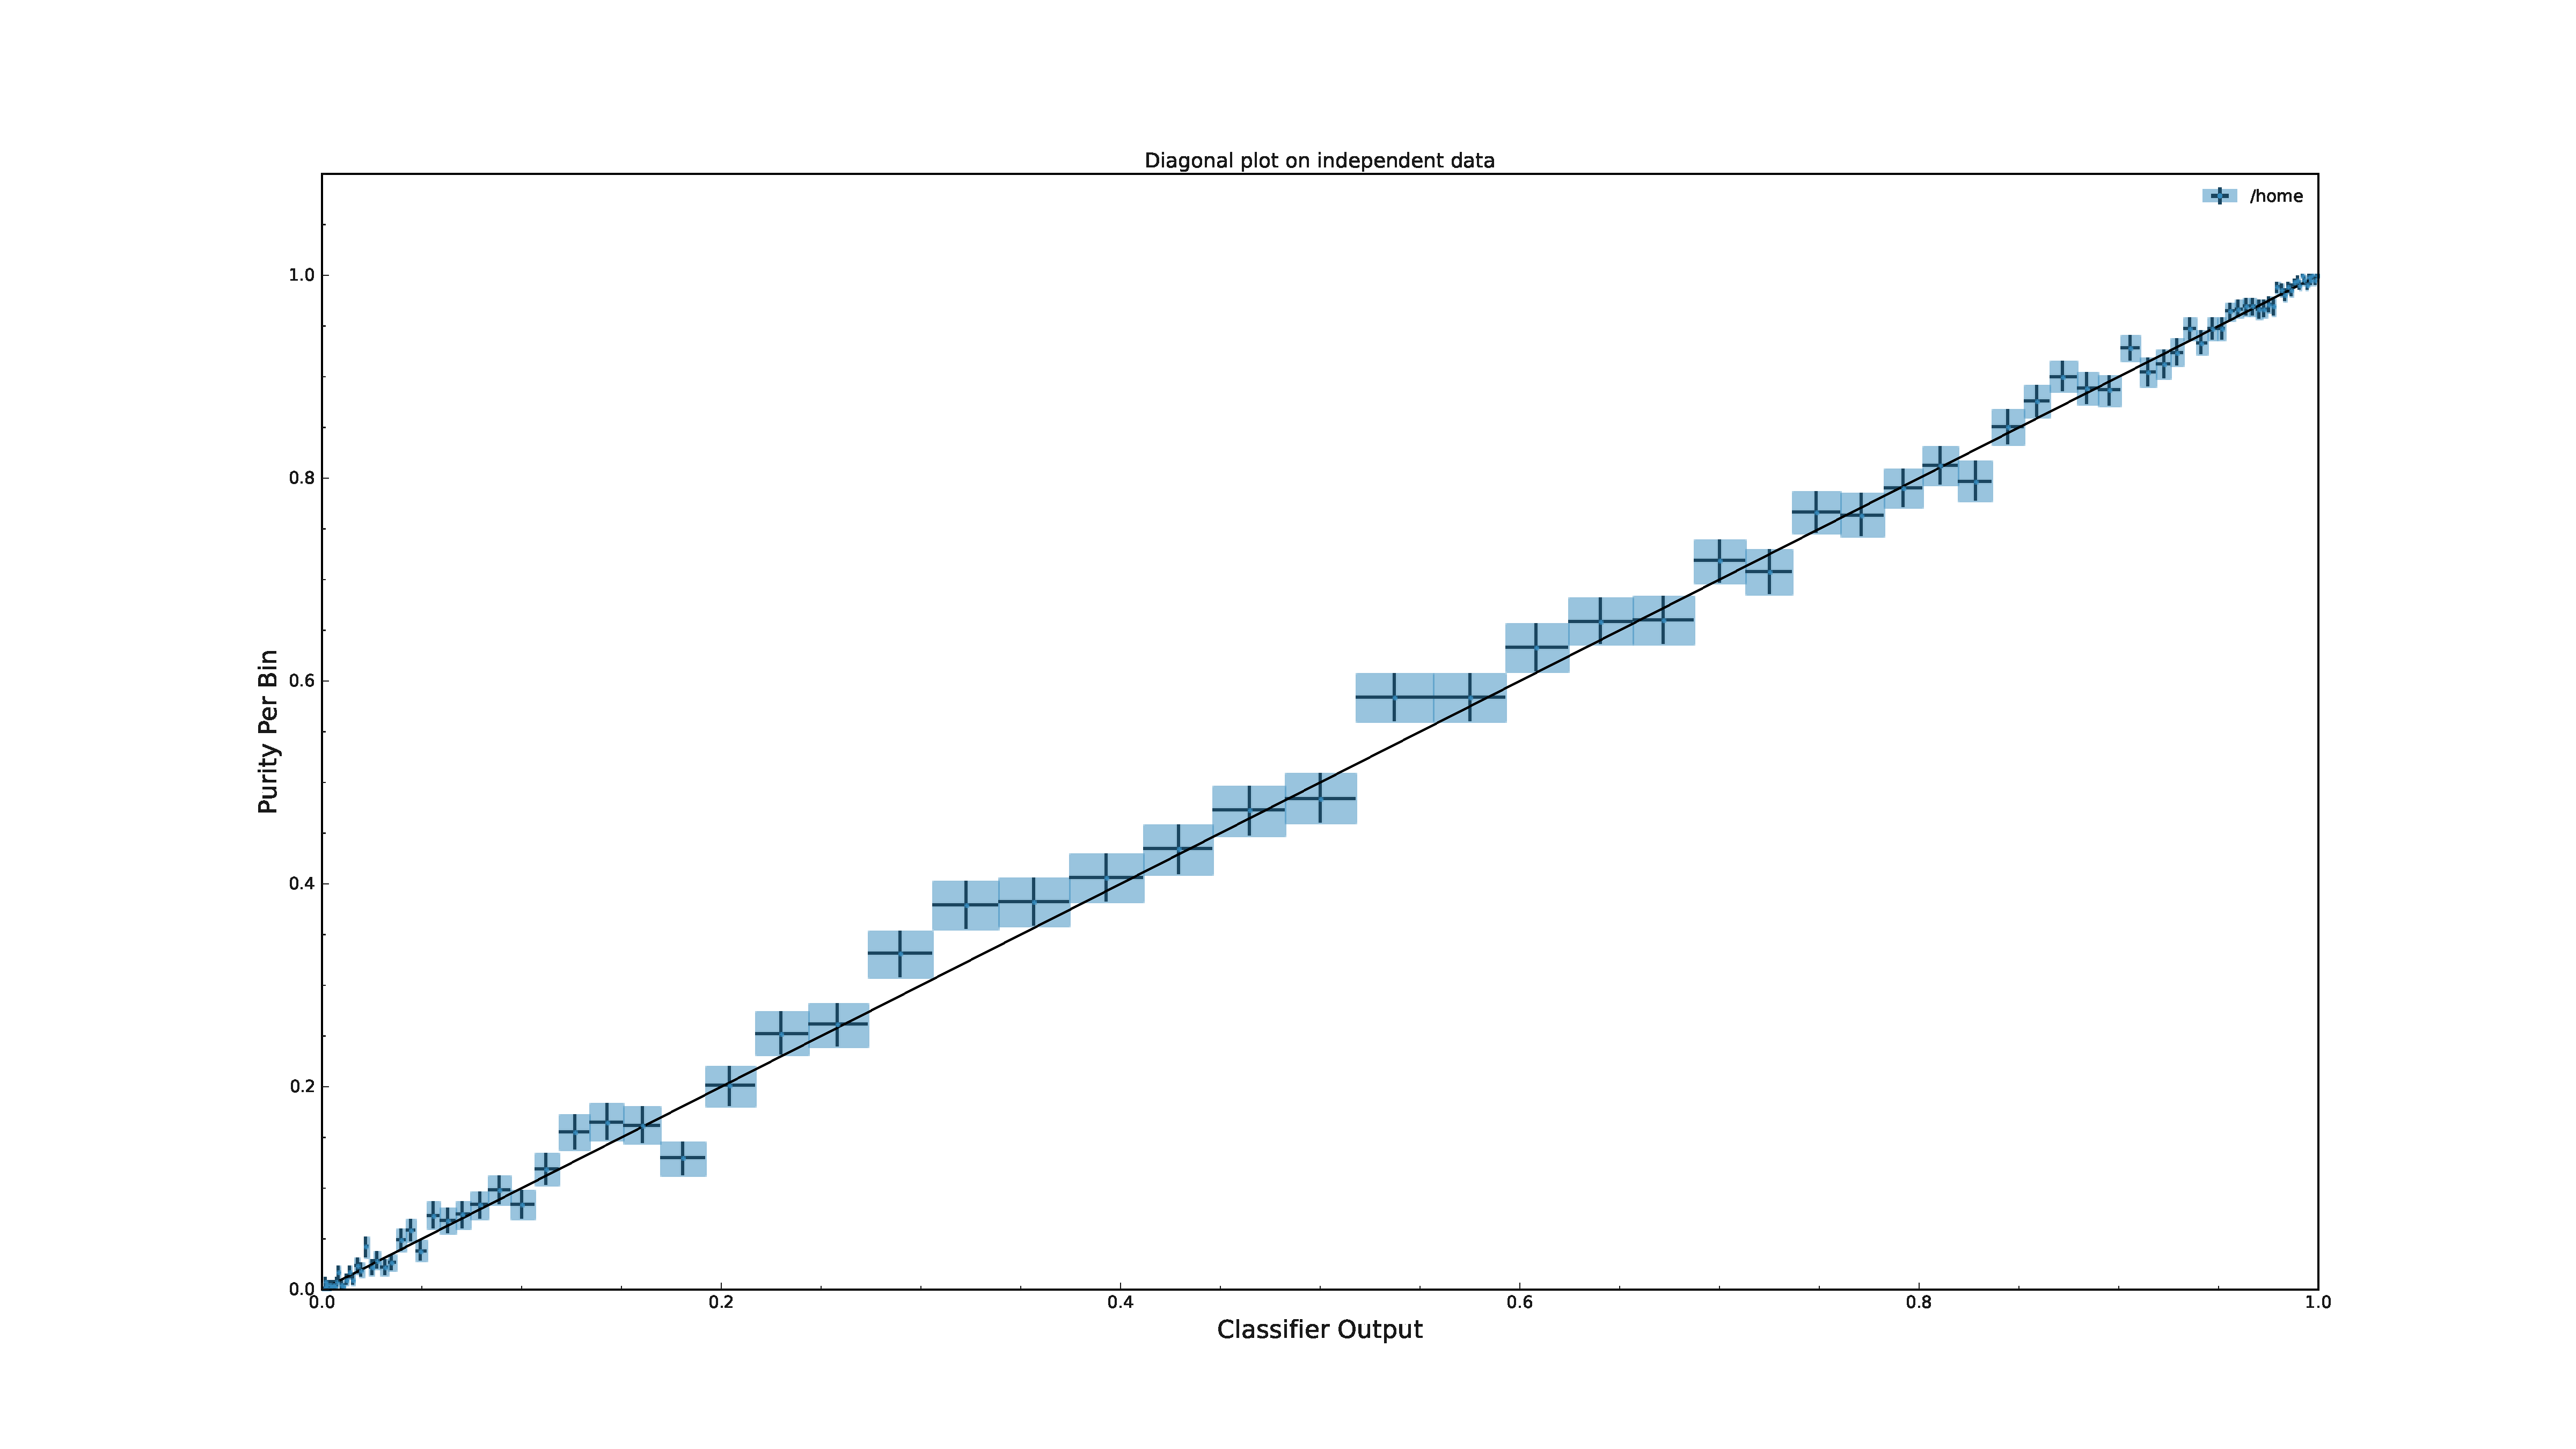
\includegraphics[width=1.0\textwidth]{evaluate_17/diagonal_plot_test.pdf}
			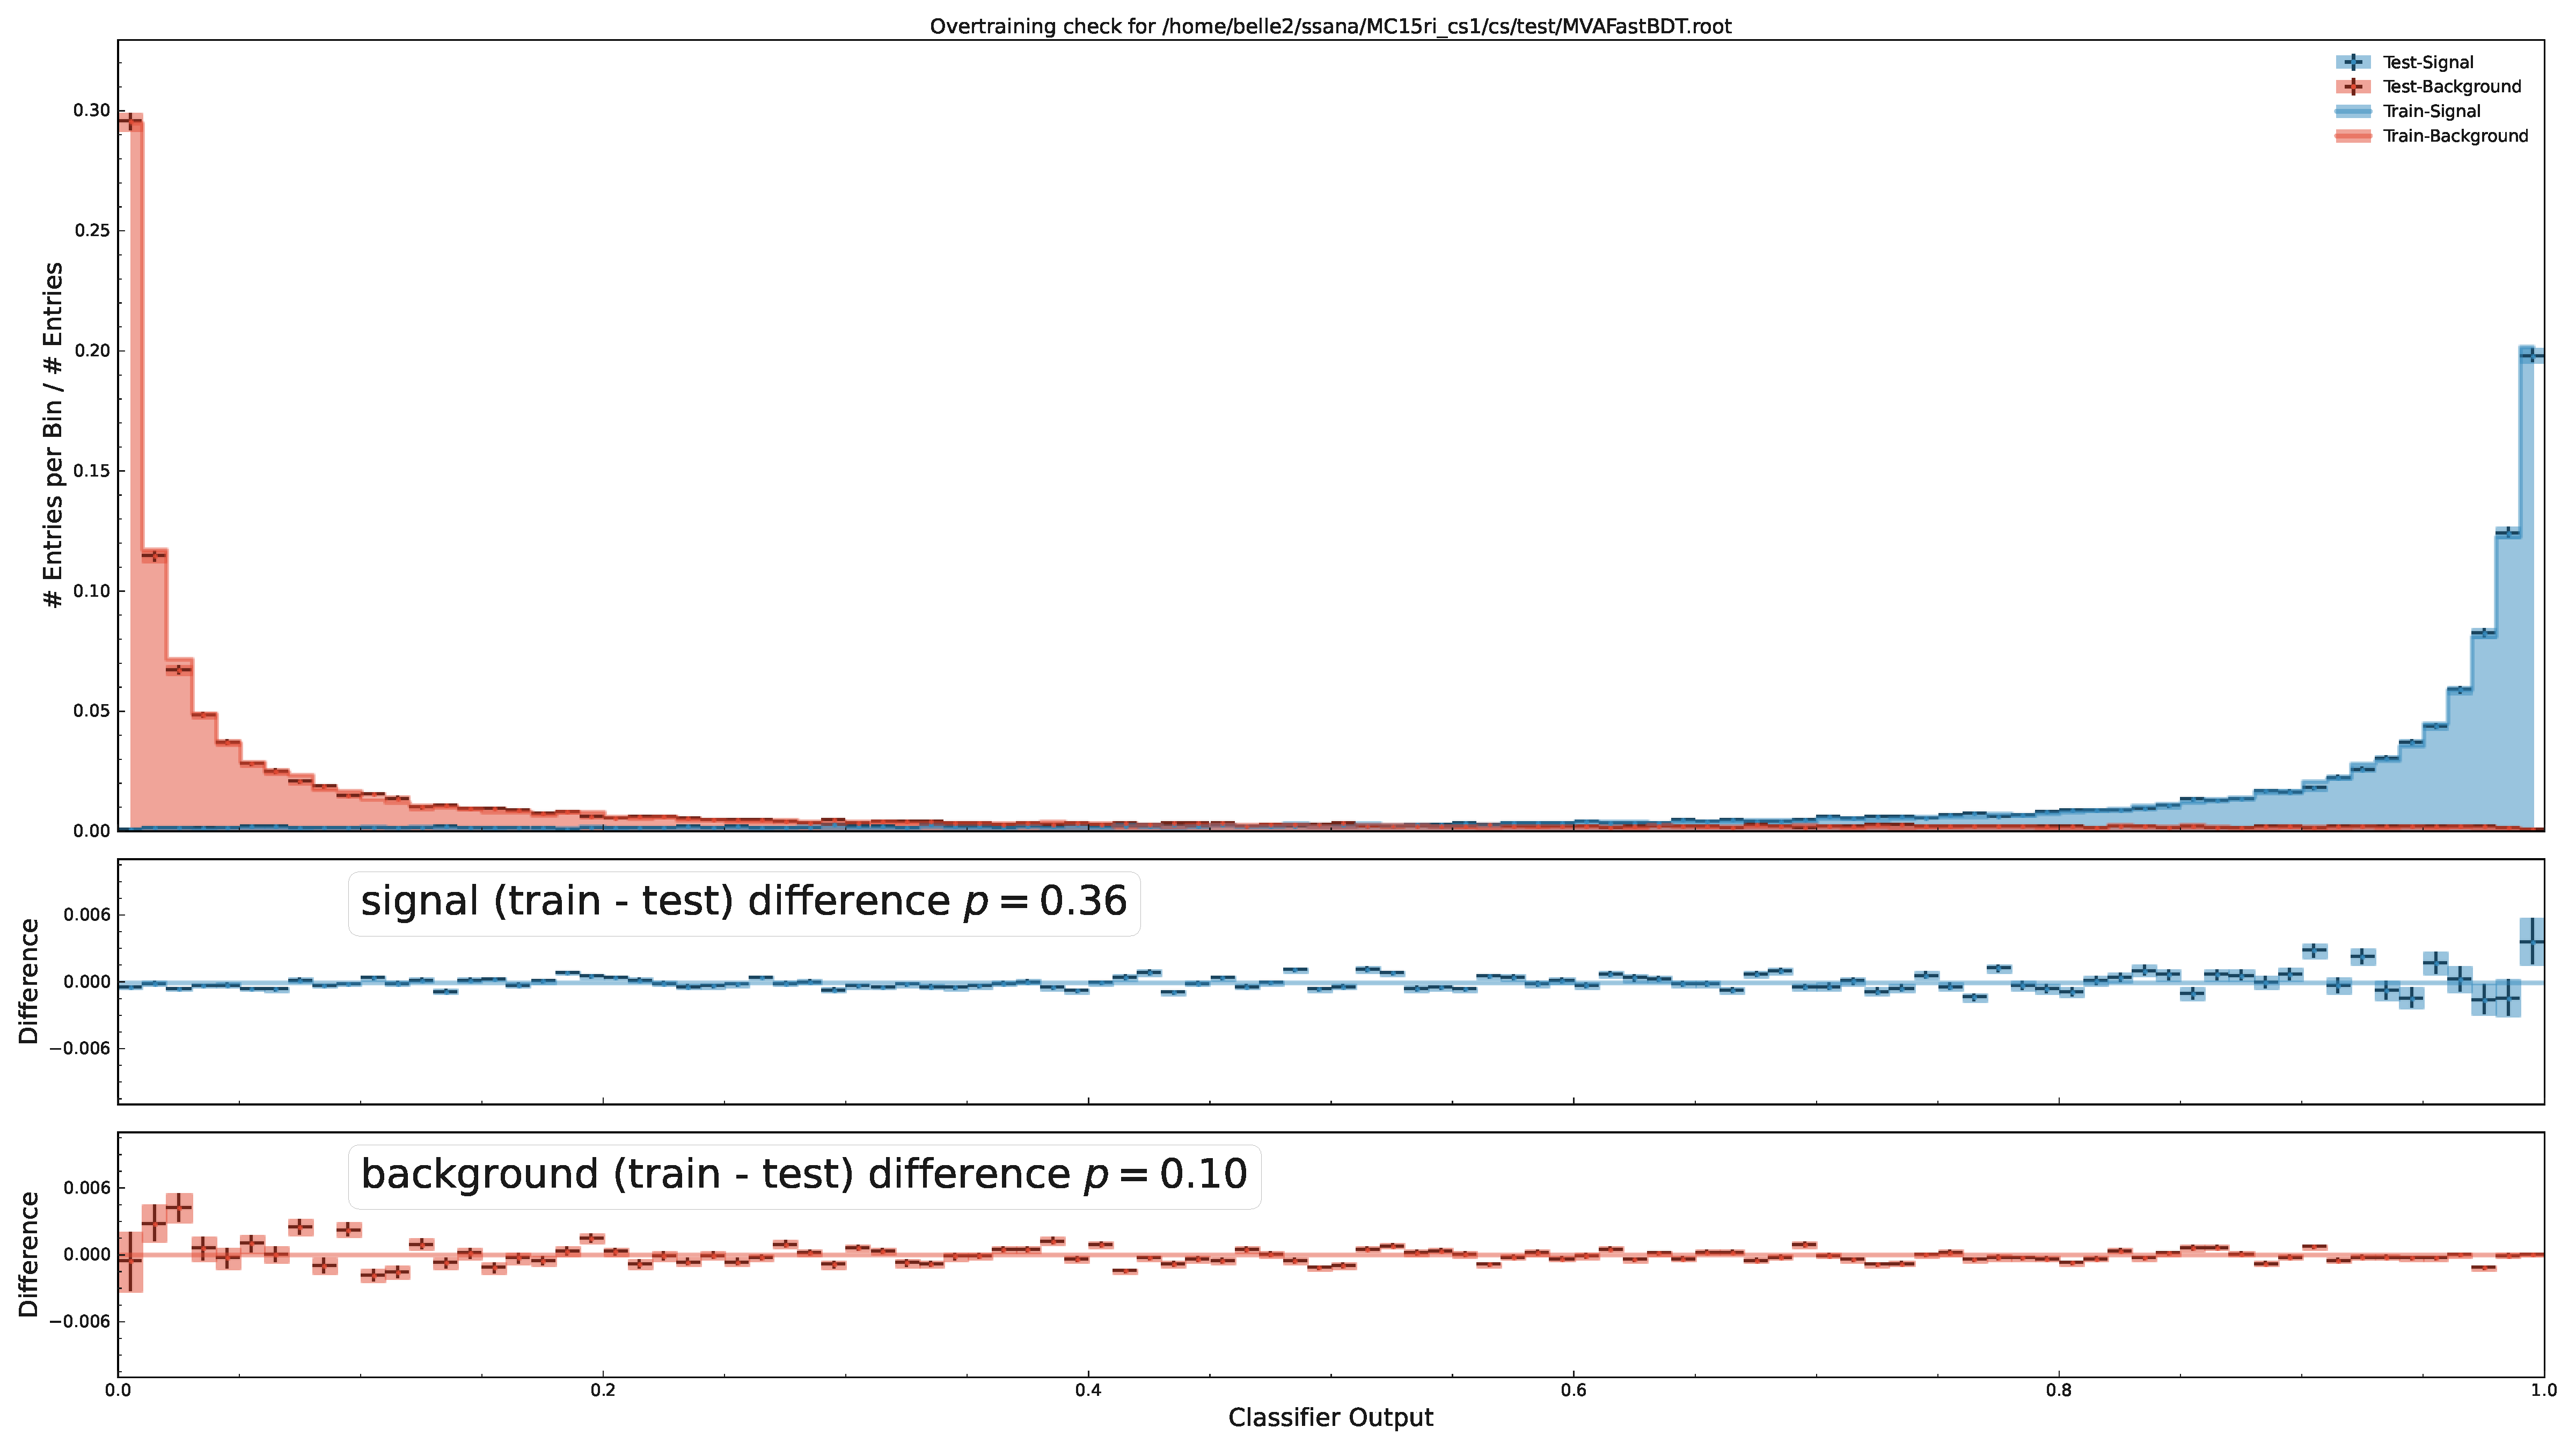
\includegraphics[width=1.0\textwidth]{evaluate_17/overtraining_plot_-936217630058450507.pdf}
		\end{figure}
		
		\column{0.3\textwidth}
		% \begin{figure}
		% 	% \vspace{-0.2 in}
		% 	% 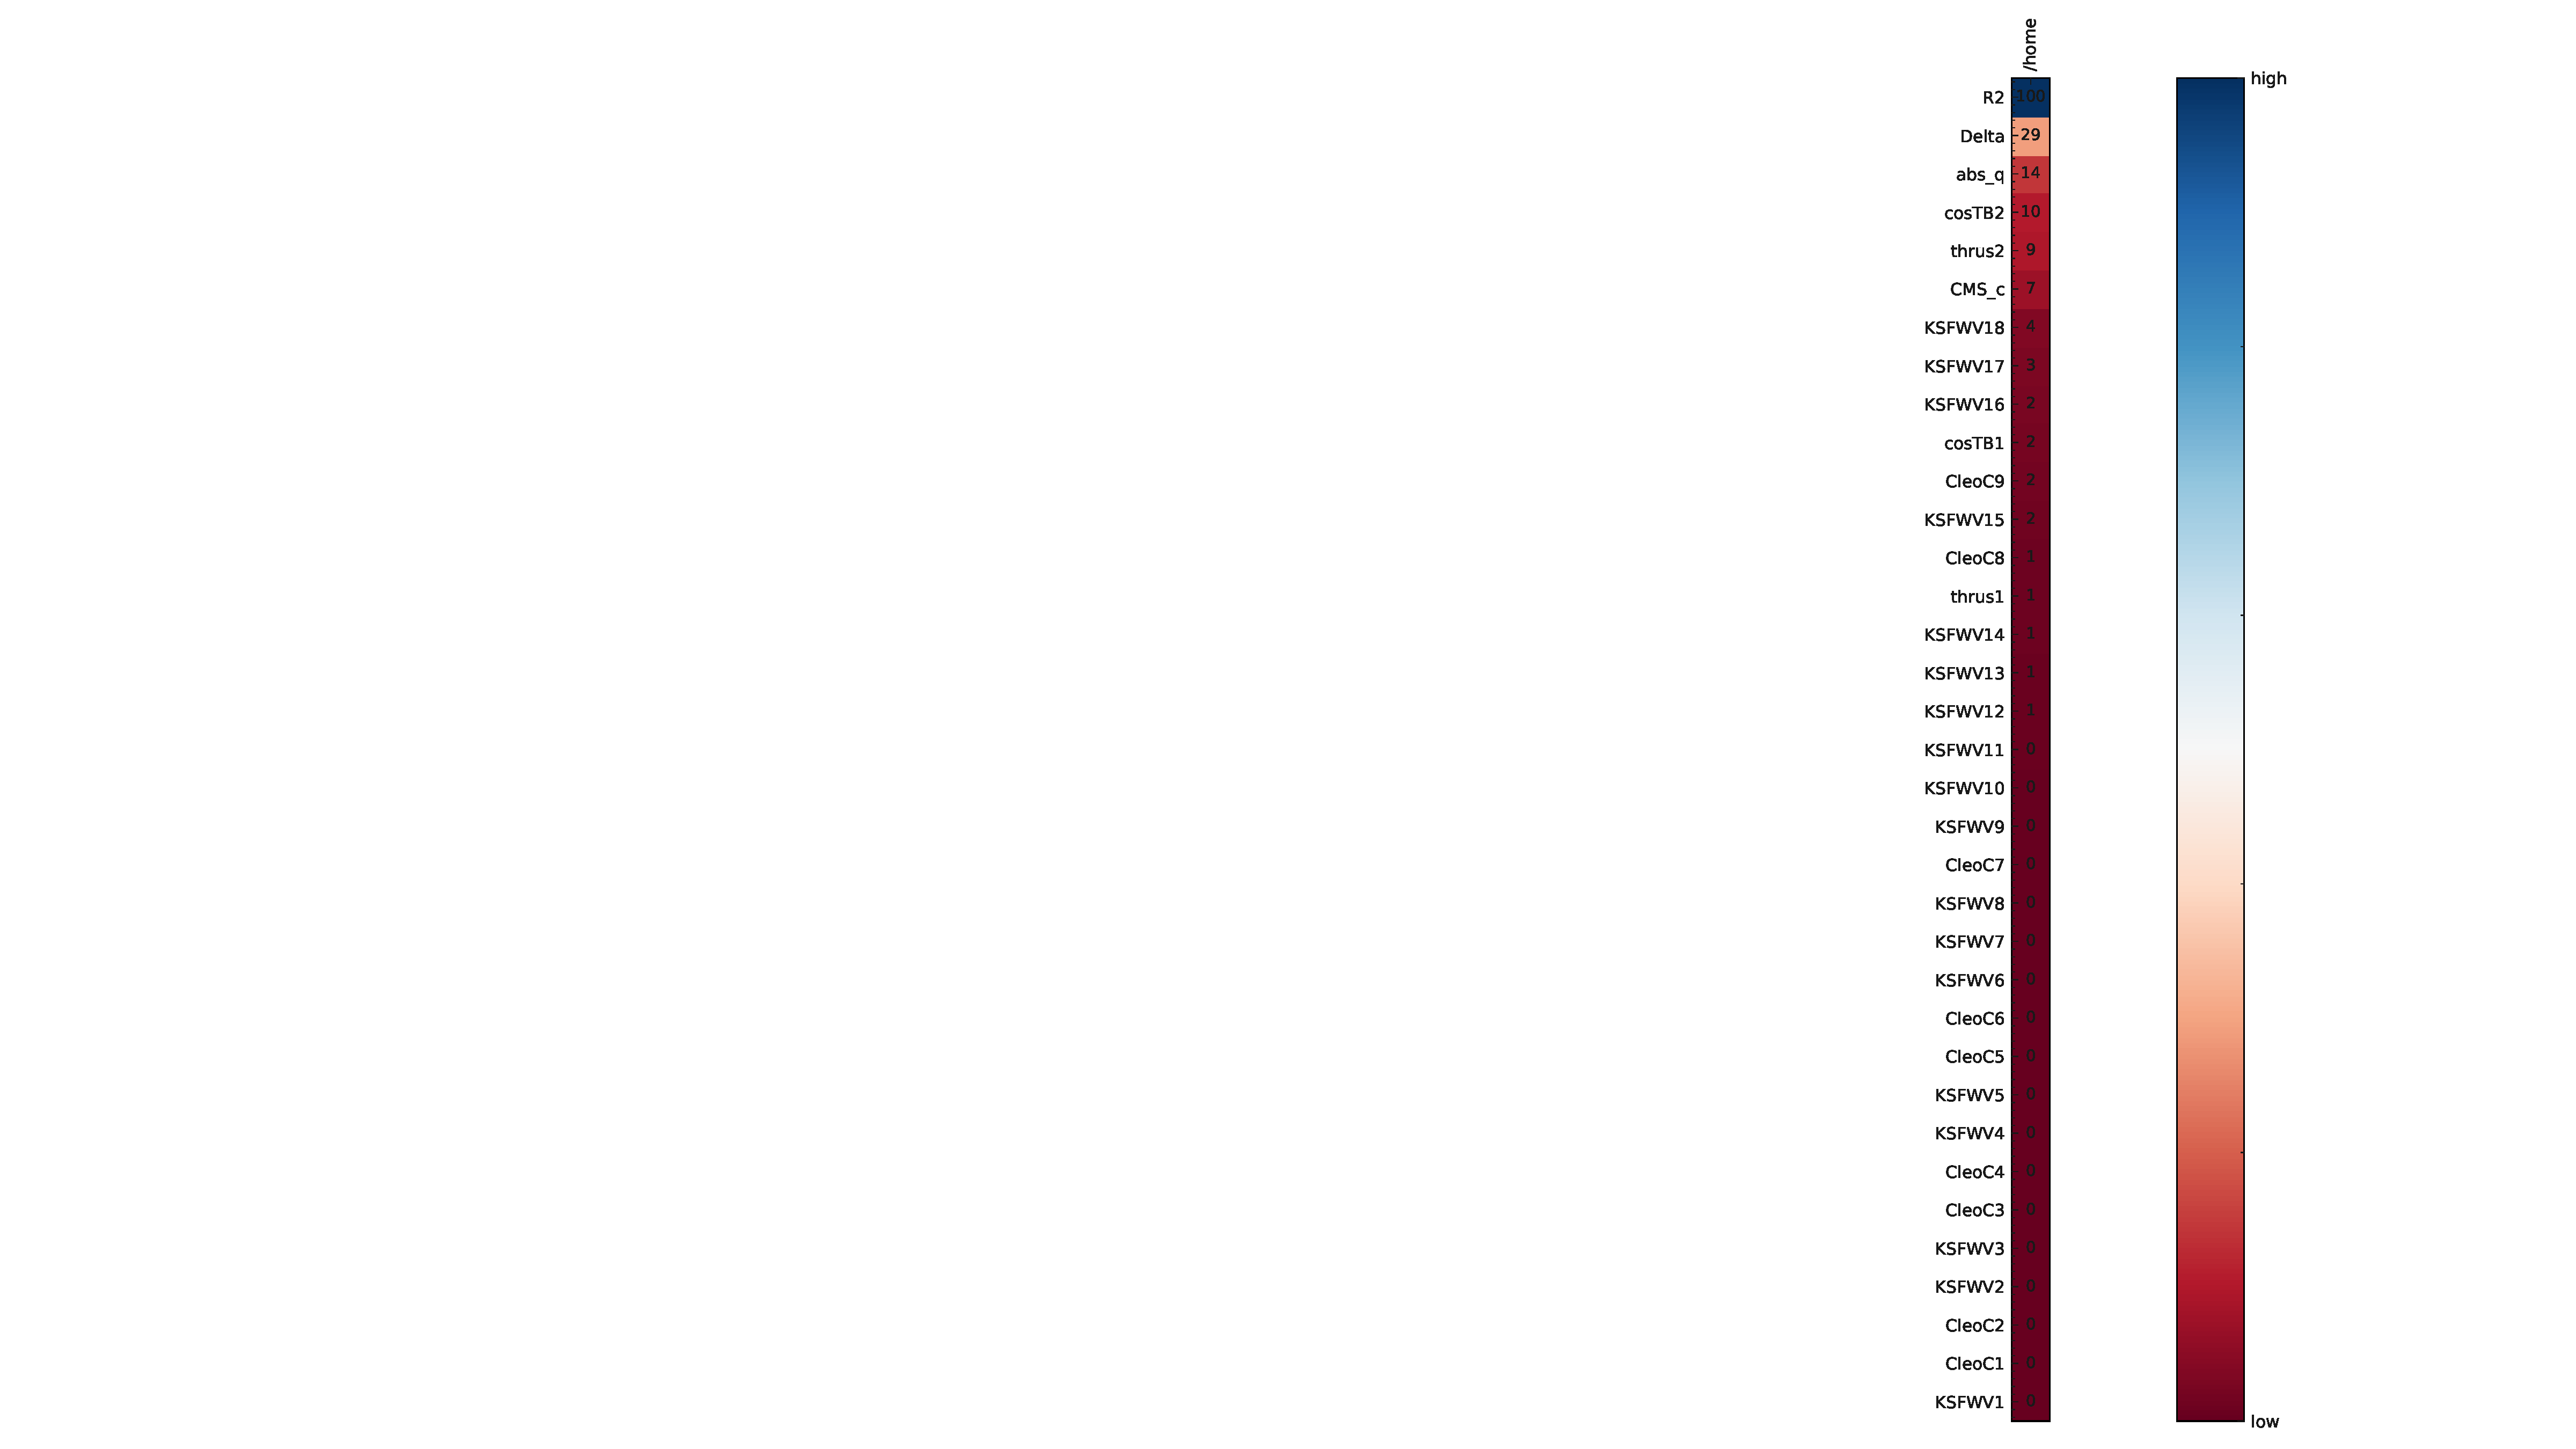
\includegraphics[width=1.0\textwidth]{evaluate_35/importance.pdf}
		% \end{figure}
	\end{columns}
\end{frame}
\begin{frame}{35 variables}
\hspace{-1in}
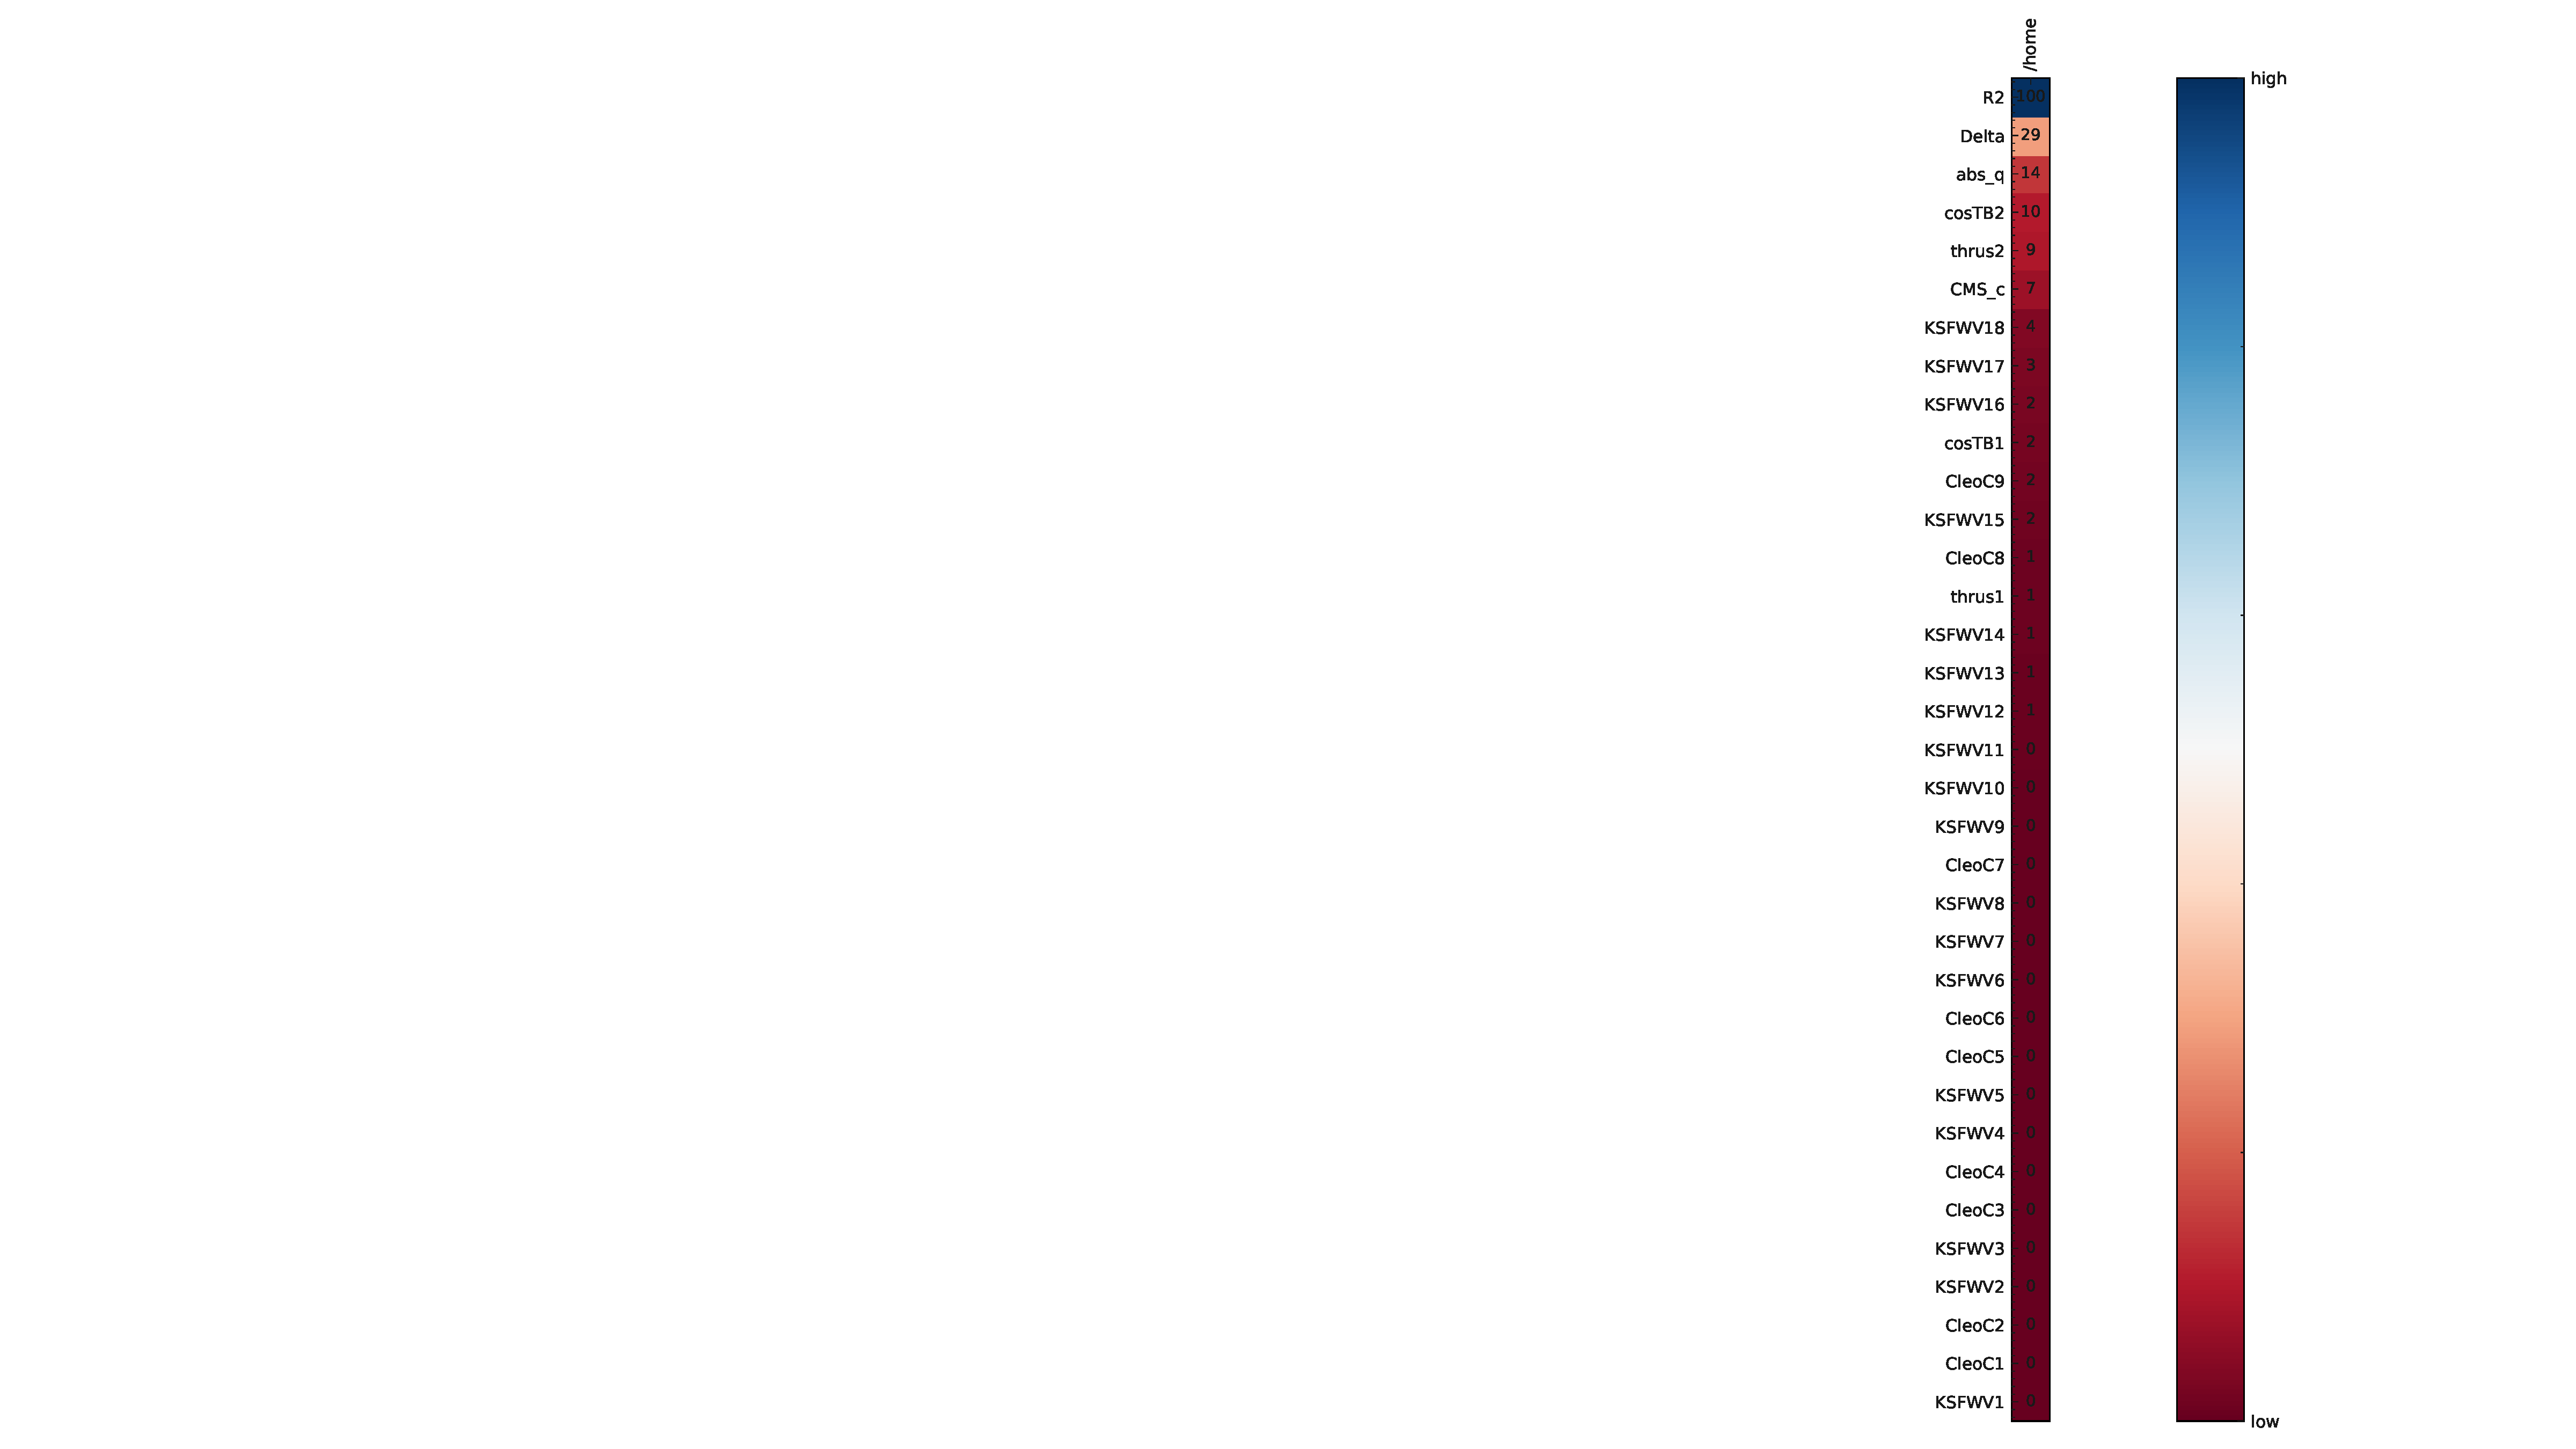
\includegraphics[width=1.25\textwidth]{evaluate_35/importance.pdf}
	\vspace{-3.3in}
	\begin{columns}
		\column{0.7\textwidth}
		\begin{figure}
			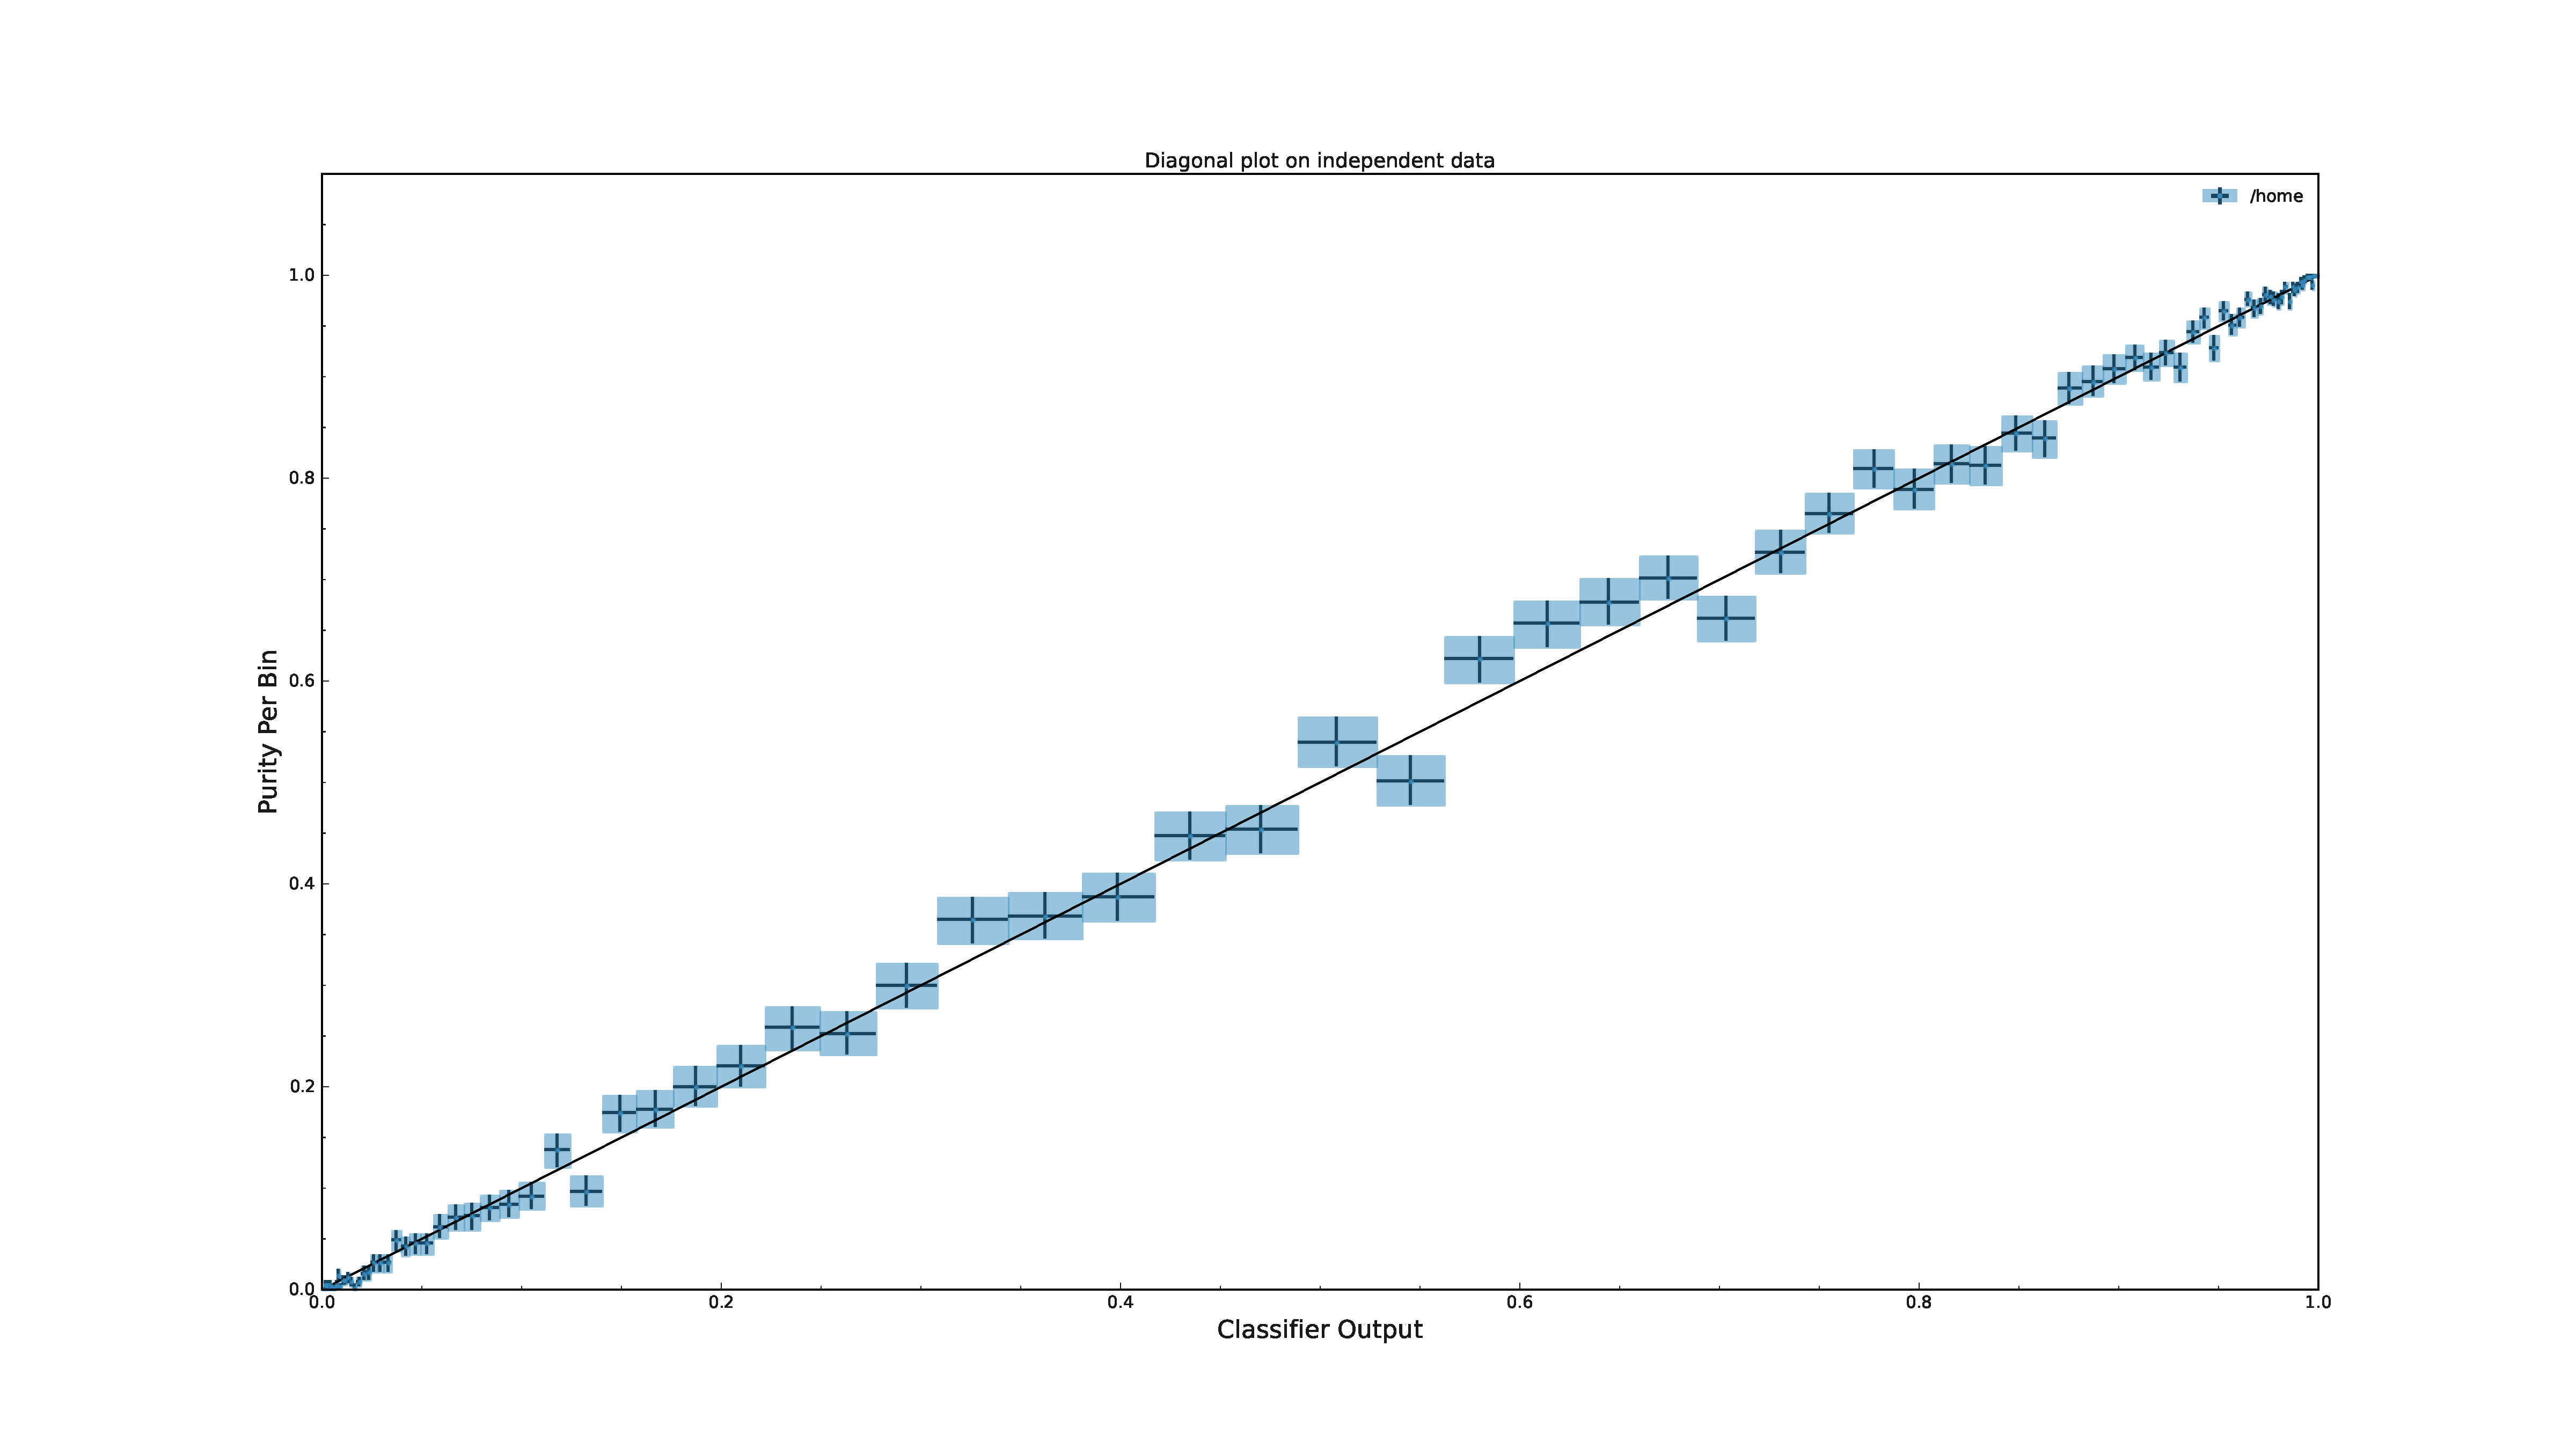
\includegraphics[width=1.0\textwidth]{evaluate_35/diagonal_plot_test.pdf}
			\includegraphics[width=1.0\textwidth]{evaluate_35/overtraining_plot_-6845103939654726996.pdf}
		\end{figure}
		
		\column{0.3\textwidth}
		% \begin{figure}
		% 	% \vspace{-0.2 in}
		% 	% 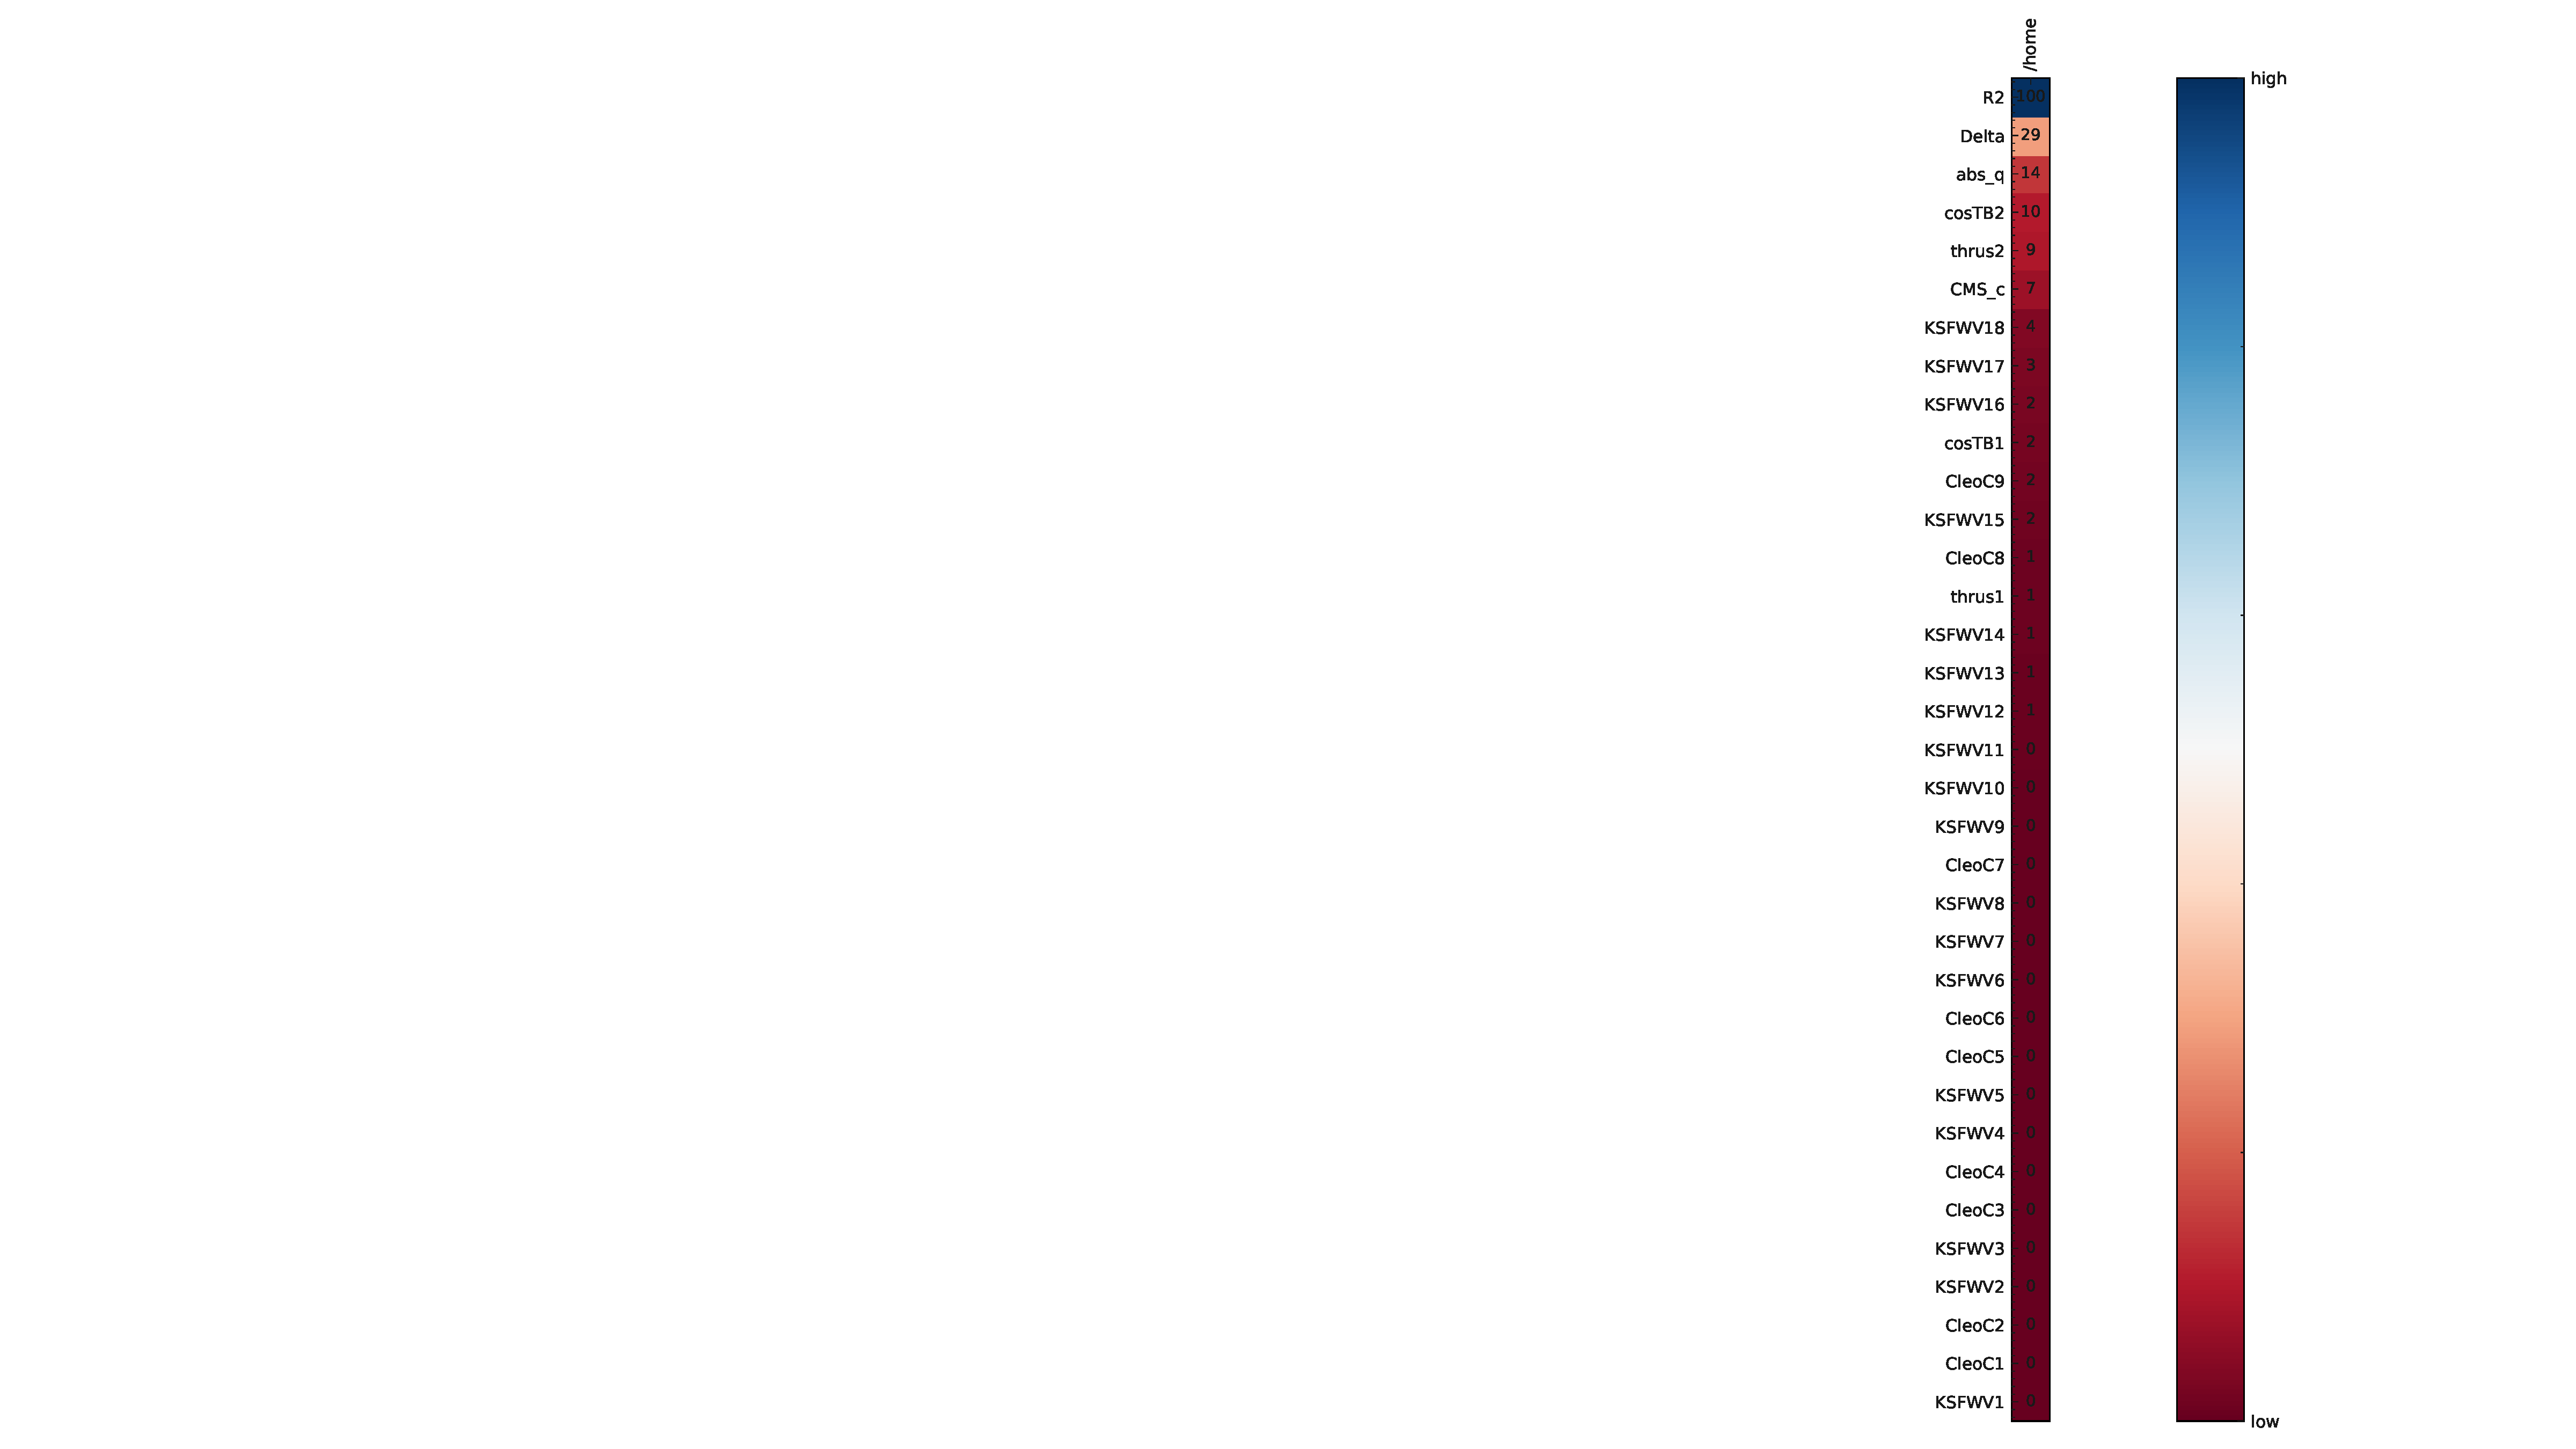
\includegraphics[width=1.0\textwidth]{evaluate_35/importance.pdf}
		% \end{figure}
	\end{columns}
\end{frame}

% \begin{frame}{}                                                                           

% \end{frame}
% \begin{frame}{} 

% \end{frame}

\end{document}
